\RequirePackage[2020-02-02]{latexrelease}  
%Version 3 October 2023
% See section 11 of the User Manual for version history
%
%%%%%%%%%%%%%%%%%%%%%%%%%%%%%%%%%%%%%%%%%%%%%%%%%%%%%%%%%%%%%%%%%%%%%%
%%                                                                 %%
%% Please do not use \input{...} to include other tex files.       %%
%% Submit your LaTeX manuscript as one .tex document.              %%
%%                                                                 %%
%% All additional figures and files should be attached             %%
%% separately and not embedded in the \TeX\ document itself.       %%
%%                                                                 %%
%%%%%%%%%%%%%%%%%%%%%%%%%%%%%%%%%%%%%%%%%%%%%%%%%%%%%%%%%%%%%%%%%%%%%

%%\documentclass[referee,sn-basic]{sn-jnl}% referee option is meant for double line spacing

%%=======================================================%%
%% to print line numbers in the margin use lineno option %%
%%=======================================================%%

%%\documentclass[lineno,sn-basic]{sn-jnl}% Basic Springer Nature Reference Style/Chemistry Reference Style

%%======================================================%%
%% to compile with pdflatex/xelatex use pdflatex option %%
%%======================================================%%

%%\documentclass[pdflatex,sn-basic]{sn-jnl}% Basic Springer Nature Reference Style/Chemistry Reference Style


%%Note: the following reference styles support Namedate and Numbered referencing. By default the style follows the most common style. To switch between the options you can add or remove �Numbered� in the optional parenthesis. 
%%The option is available for: sn-basic.bst, sn-vancouver.bst, sn-chicago.bst%  
 
\documentclass[sn-nature]{sn-jnl}% Style for submissions to Nature Portfolio journals
%%\documentclass[sn-basic]{sn-jnl}% Basic Springer Nature Reference Style/Chemistry Reference Style
%%\documentclass[bst/sn-mathphys-num]{sn-jnl}% Math and Physical Sciences Numbered Reference Style 
%%\documentclass[sn-mathphys-ay]{sn-jnl}% Math and Physical Sciences Author Year Reference Style
%%\documentclass[sn-aps]{sn-jnl}% American Physical Society (APS) Reference Style
%%\documentclass[sn-vancouver,Numbered]{sn-jnl}% Vancouver Reference Style
%%\documentclass[sn-apa]{sn-jnl}% APA Reference Style 
%%\documentclass[sn-chicago]{sn-jnl}% Chicago-based Humanities Reference Style


%bib2
%%%% Standard Packages
%%<additional latex packages if required can be included here>

\usepackage{graphicx}%
\usepackage{multirow}%
\usepackage{amsmath,amssymb,amsfonts}%
\usepackage{amsthm}%
\usepackage{mathrsfs}%
\usepackage[title]{appendix}%
\usepackage{xcolor,placeins}%
\usepackage{textcomp}%
\usepackage{manyfoot}%
\usepackage{booktabs}%
\usepackage{algorithm}%
\usepackage{algorithmicx}%
\usepackage{algpseudocode}%
\usepackage{listings}%
\usepackage{environ, etoolbox}
\usepackage{amsthm, siunitx} % For math fonts, symbols and environments
%%%%

%%%%%=============================================================================%%%%
%%%%  Remarks: This template is provided to aid authors with the preparation
%%%%  of original research articles intended for submission to journals published 
%%%%  by Springer Nature. The guidance has been prepared in partnership with 
%%%%  production teams to conform to Springer Nature technical requirements. 
%%%%  Editorial and presentation requirements differ among journal portfolios and 
%%%%  research disciplines. You may find sections in this template are irrelevant 
%%%%  to your work and are empowered to omit any such section if allowed by the 
%%%%  journal you intend to submit to. The submission guidelines and policies 
%%%%  of the journal take precedence. A detailed User Manual is available in the 
%%%%  template package for technical guidance.
%%%%%=============================================================================%%%%

%% as per the requirement new theorem styles can be included as shown below
\theoremstyle{thmstyleone}%
\newtheorem{theorem}{Theorem}%  meant for continuous numbers
%%\newtheorem{theorem}{Theorem}[section]% meant for sectionwise numbers
%% optional argument [theorem] produces theorem numbering sequence instead of independent numbers for Proposition
\newtheorem{proposition}[theorem]{Proposition}% 
%%\newtheorem{proposition}{Proposition}% to get separate numbers for theorem and proposition etc.
\newcommand\eref[1]{{\textbf{\textit{Equation \ref{#1}}}}{}}                                                                                                                        
\newcommand\erefs[2]{\textbf{\textit{Equations \ref{#1} \& \ref{#2}}}}                                                                                                              
\newcommand\fref[1]{\normalsize{\textbf{\textit{Figure \ref{#1}}}}\normalsize{}}                                                                                                    
\newcommand\dref[2]{\normalsize{\textbf{\textit{Figure \ref{#1}#2}}}\normalsize{}}                                                                                                  
\newcommand\sref[1]{\normalsize{\textbf{\textit{Supplemental Figure \ref{#1}}}}\normalsize{}}                                                                                       
\newcommand\tref[1]{\normalsize{\textbf{\textit{Table \ref{#1}}}}\normalsize{}}                                                                                                     
\newcommand\need[1]{\textbf{\textcolor{red}{NEED: #1}}}                                                                                                                             
\newtoggle{showFig}
\togglefalse{showFig} \toggletrue{showFig}
\NewEnviron{maybe}[1]{\iftoggle{#1}{\BODY}{}}




\theoremstyle{thmstyletwo}%
\newtheorem{example}{Example}%
\newtheorem{remark}{Remark}%

\theoremstyle{thmstylethree}%
\newtheorem{definition}{Definition}%

\raggedbottom
%%\unnumbered% uncomment this for unnumbered level heads

\begin{document}

\title[Article Title]{Article Title}

\title[Article Title]{Striking Departure from Polygenic Architecture in the Tails of Complex Traits}

%%=============================================================%%
%% GivenName	-> \fnm{Joergen W.}
%% Particle	-> \spfx{van der} -> surname prefix
%% FamilyName	-> \sur{Ploeg}
%% Suffix	-> \sfx{IV}
%% \author*[1,2]{\fnm{Joergen W.} \spfx{van der} \sur{Ploeg} 
%%  \sfx{IV}}\email{iauthor@gmail.com}
%%=============================================================%%

\author*[1,2]{\fnm{First} \sur{Author}}\email{iauthor@gmail.com}

\author[2,3]{\fnm{Second} \sur{Author}}\email{iiauthor@gmail.com}
\equalcont{These authors contributed equally to this work.}

\author[1,2]{\fnm{Third} \sur{Author}}\email{iiiauthor@gmail.com}
\equalcont{These authors contributed equally to this work.}

\affil*[1]{\orgdiv{Department}, \orgname{Organization}, \orgaddress{\street{Street}, \city{City}, \postcode{100190}, \state{State}, \country{Country}}}

\affil[2]{\orgdiv{Department}, \orgname{Organization}, \orgaddress{\street{Street}, \city{City}, \postcode{10587}, \state{State}, \country{Country}}}

\affil[3]{\orgdiv{Department}, \orgname{Organization}, \orgaddress{\street{Street}, \city{City}, \postcode{610101}, \state{State}, \country{Country}}}

%%==================================%%
%% Sample for unstructured abstract %%
%%==================================%%

\abstract{Understanding the genetic architecture of human traits is a key goal 
of biomedical research and precision medicine.  However, little is known about 
how genetic architecture varies across the trait continuum and, in particular, 
if it differs in the tails of complex traits, where disease often occurs. Here, applying an approach that 
utilizes polygenic scores, we observe striking evidence of pervasive and substantial departures in polygenic 
architecture across 148 complex trait tails (e.g. bottom/top 1\% of LDL, BMI, glucose) tested in UK Biobank data. 
These results replicate in individuals with repeat measures, in non-European UKB individuals, 
in the US-based All Of Us dataset, and in our sibling-based test of tail architecture. We demonstrate that 
PRSs perform relatively poorly in tails with reduced polygenic architecture and that those tails are associated 
with enrichment of rare alleles and advanced paternal age. Finally, we find evidence of ongoing 
selection consistent with observed departures in polygenicity and demonstrate, via simulation, 
that trait tails under selective pressure are expected to be enriched for rare, large-effect alleles2. 
Therefore, a substantial fraction of individuals may have extreme trait values due to only one or 
several alleles of very large effect, rather than polygenic burden. Overall, our findings suggest that 
selection can drive distinct genetic architecture in the tails of complex traits. Our study has implications 
for the discovery of rare variants, for the utility of polygenic scores and for the relative importance 
of common and rare variants to human traits and disease.}



%%================================%%
%% Sample for structured abstract %%
%%================================%%

% \abstract{\textbf{Purpose:} The abstract serves both as a general introduction to the topic and as a brief, non-technical summary of the main results and their implications. The abstract must not include subheadings (unless expressly permitted in the journal's Instructions to Authors), equations or citations. As a guide the abstract should not exceed 200 words. Most journals do not set a hard limit however authors are advised to check the author instructions for the journal they are submitting to.
% 
% \textbf{Methods:} The abstract serves both as a general introduction to the topic and as a brief, non-technical summary of the main results and their implications. The abstract must not include subheadings (unless expressly permitted in the journal's Instructions to Authors), equations or citations. As a guide the abstract should not exceed 200 words. Most journals do not set a hard limit however authors are advised to check the author instructions for the journal they are submitting to.
% 
% \textbf{Results:} The abstract serves both as a general introduction to the topic and as a brief, non-technical summary of the main results and their implications. The abstract must not include subheadings (unless expressly permitted in the journal's Instructions to Authors), equations or citations. As a guide the abstract should not exceed 200 words. Most journals do not set a hard limit however authors are advised to check the author instructions for the journal they are submitting to.
% 
% \textbf{Conclusion:} The abstract serves both as a general introduction to the topic and as a brief, non-technical summary of the main results and their implications. The abstract must not include subheadings (unless expressly permitted in the journal's Instructions to Authors), equations or citations. As a guide the abstract should not exceed 200 words. Most journals do not set a hard limit however authors are advised to check the author instructions for the journal they are submitting to.}

\keywords{keyword1, Keyword2, Keyword3, Keyword4}

%%\pacs[JEL Classification]{D8, H51}

%%\pacs[MSC Classification]{35A01, 65L10, 65L12, 65L20, 65L70}

\maketitle






%%%%%%%%%%%%%%%%%%%%%%%%%%%%%%%%%%%%%%%%%%%%%%%%%%%%%%%%%%%%%%%%%%%%%%%%%%%%%%%
%%%%%%%%%%%%%%%%%%%%%%%%%%%%%%%%%%%   INTRO    %%%%%%%%%%%%%%%%%%%%%%%%%%%%%%%%
%%%%%%%%%%%%%%%%%%%%%%%%%%%%%%%%%%%%%%%%%%%%%%%%%%%%%%%%%%%%%%%%%%%%%%%%%%%%%%%

\section{Introduction}\label{sec1}

%The Introduction section, of referenced text \cite{bib1} expands on the 
%background of the work (some overlap with the Abstract is acceptable). 
%The introduction should not include subheadings.
%Springer Nature does not impose a strict layout as standard however authors are 
%advised to check the individual requirements for the journal they are planning 
%to submit to as there may be journal-level preferences. When preparing your 
%text please also be aware that some stylistic choices are not supported in full 
%text XML (publication version), including coloured font. These will not be 
%replicated in the typeset article if it is accepted. 

Background to genetic architecture, detection of variants and theory/methods relating to polygenicity. 
Also something on selection shaping genetic variation / polygenicity etc. End on the gap, despite all this, 
it's unknown how GA varies across trait continuum 
(and the role that selection might play in that) / + as a result, we don't have a way of inferring 
whether an individual has a rare/common cause. 


We introduce a method that utilizes polygenic risk scores (PRS) to detect departures from polygenic 
architecture in trait tails from population data: the PRS-On-Phenotype outlier ("POPout") test. 
Explain how it works. Say that we apply this to UKB and All of US data. Also explain that we've 
already developed a sibling-based test to do this as well.


Some flavour of the results. Also elaborate a bit on the selection work.. done to help explain the 
observations and to set them in the context of how pop gen processes produce the genetic variation 
and how it manifests (cite a lot of the selection work on this), or maybe this whole paragraph 
could focus on the involvement/explanation of selection here. 




\section*{Old Introduction} 

Complex polygenic traits are typically modeled as the additive sum of 
many variants of limited effect alongside rare risk alleles of substantial 
penetrence. This distinction likely reflects a balance between long-range 
selection pressure and the limited ability of trait-altering 
mutant alleles to persist over multiple generations.  Identification of individuals with extreme trait values as  
probable carriers of rare high-impact variants has led sequencing strategies to focus on individuals in the tails 
of the trait distribution.  Tail trait values can also result from extreme polygenic burden created by 
recombination and reassortment.  Therefore, to enhance the efficency of sequencing studies, 
it is imperative to be able to discriminate between these different etiologies.  
    
One indicatation that rare variants may play a significant role in the
tails of the trait distribution can be reflected in the reliability of
polygenic risk scores (PRS) in the tails.  If highly penetrant rare
variants not included in GWAS determine the tails of the trait
distribution such individuals will not be assigned appropriate risk
scores.  In this study, we develop a \textit{polygenic
  regression-to-mean} (PRM) statistical test that compares the PRS in
the tails of the trait distribution to expectation PRS under a
polygenic model.  Applying this test to hundreds of traits in the UK
Biobank reveals that the majority of quantitive traits exhibit
significant PRM in one or both tails.

Next we examine whether rare variants in exome studies are enriched in trait tails with significant tail 
regression and demonstrate that such tails are more likely to be under negative selection.  Further examining 
these trait tails we find an association between PRM and other measures of fitness that may be influenced by rare 
variants including the lifetime number of illnesses and still births.  We then compare these 
results to a simulation and find that they match. 

Finally, we assess whether the predictions of a complex trait architecture derived from a conditional sibling 
model align with the observed diversity in the architecture of trait extremes. The concordance between these measures underscores the need to 
consider the role of rare variants in the analysis of trait tails.  The PRS and sibling analyses presented here 
offer valuable tools for the targeted selection of traits and samples likely to harbor de novo or rare 
deleterious alleles and represent an approach that has the potential to significantly enhance the 
effectiveness and design of sequencing studies.
Genome-wide association studies (GWAS) are instrumental in
understanding the genetic architecture of complex traits.  These
studies typically identify numerous common genetic variants, each of
small individual effect \citep{gwas} that can be used in summation to
make predictions. The idea that these common variants adequately
represent the genetic architecture is supported by evolutionary
theory, which suggests that many human traits (e.g., height, birth
weight) are under stabilizing selection, which reduces the fitness
impact of large-effect variants \citep{v_select}.

A recent hope for advancing personalized medicine is in the potential
of polygenic risk scores to identify high-risk individuals who may
benefit from early interventions, such as adoption of specific
lifestyle regimes or increased screening \citep{bt_7, bt_8, bt_9,
  bt_10}.  However, this strategy will be underpowered when applied to
traits or diseases with reduced PRS in the tail of the distribution
due to reduced common polygenicity. To overcome this problem, the
genetic aetiology underlying the tails of phenotype distributions must
be investigated and better characterized \citep{bt_1}.  Polygenic
prediction models use these common small-effect variants to generate
polygenic risk scores (PRS) whose performance making out-of-sample
predictions is usually evaluated with aggregate estimates like
\emph{variance explained} ($R^2$).  However, new evidence has
suggested that this level of analysis may not be adequate because the
preformance of prediction models is not uniform across the trait
distribution.  This non-uniformity results because the contribution of
small effect common variants relative to highly penetrant rare
variants and the environment is not equal across the trait
distribution \citep{bt_1, bt_2}.

This negative correlation between effect size and minor allele
frequency (MAF) reflects the interplay between long term selection against
extreme trait values and the ability of mutant alleles with
significant effects to escape this trend through chance or short term
environmental changes. Recent or ongoing selection can leave distinct
genetic signatures, such as an enrichment of rare variants in
individuals in the tails of trait distributions during directional or
stabilizing selection. The expectation that individuals with extreme
trait values are more likely to carry rare large-effect variants has
led to strategies that priorize sequencing of individuals in the tails
of the trait distribution \citep{bt_3, bt_4}.  However, tail trait
values can also result from extreme polygenic burden created by
recombination and reassortment, and a more efficient approach would
involve considering more lines of individuals to allow the selection
of individuals with strongest evidence of rare variant architecture
for sequencing.

Here we attempt to distinguish whether the tails of the distribution
of different traits are primarily driven by common polygenicity or by
a more "monogenic-type" architecture \need{monogenic literally means
  single-gene disorder}.  We accomplish this by developing a
statistical test that measures the fit of the polygenic model across
the trait-PRS distribution and identifies non-polygencity in each tail
and applying it to over a \need{thousand} UK Biobank traits (see
\fref{fig:intro}) \need{sentence is too long and "trait-PRS
  distribution" is inaccurate description}.  Next we consider whether
evidence of negative selection exists in a subset of uncorrelated
traits \need{we use all 75 traits, these are not uncorrelated}
and show that the trait tails under negative selection are more
likely to be associated with \need{PRS regression to the mean which
  may imply existence of rare variants}.  We further triangulate
evidence for selective constraint leading to reduced contribution of common
polygenicity in the tails, by testing for the associations between
known measures of fitness and PRS regression to the mean in the tails. \citep{bt_5, bt_6}.

Finally, we assess whether the predictions of a complex
trait architecture derived from a conditional sibling model align with
the observed diversity in the architecture of trait extremes inferred
from population level analyses.
































\section{Results}\label{sec2}

\FloatBarrier \begin{figure}[!h] \begin{maybe}{showFig}
\centering
\centerline{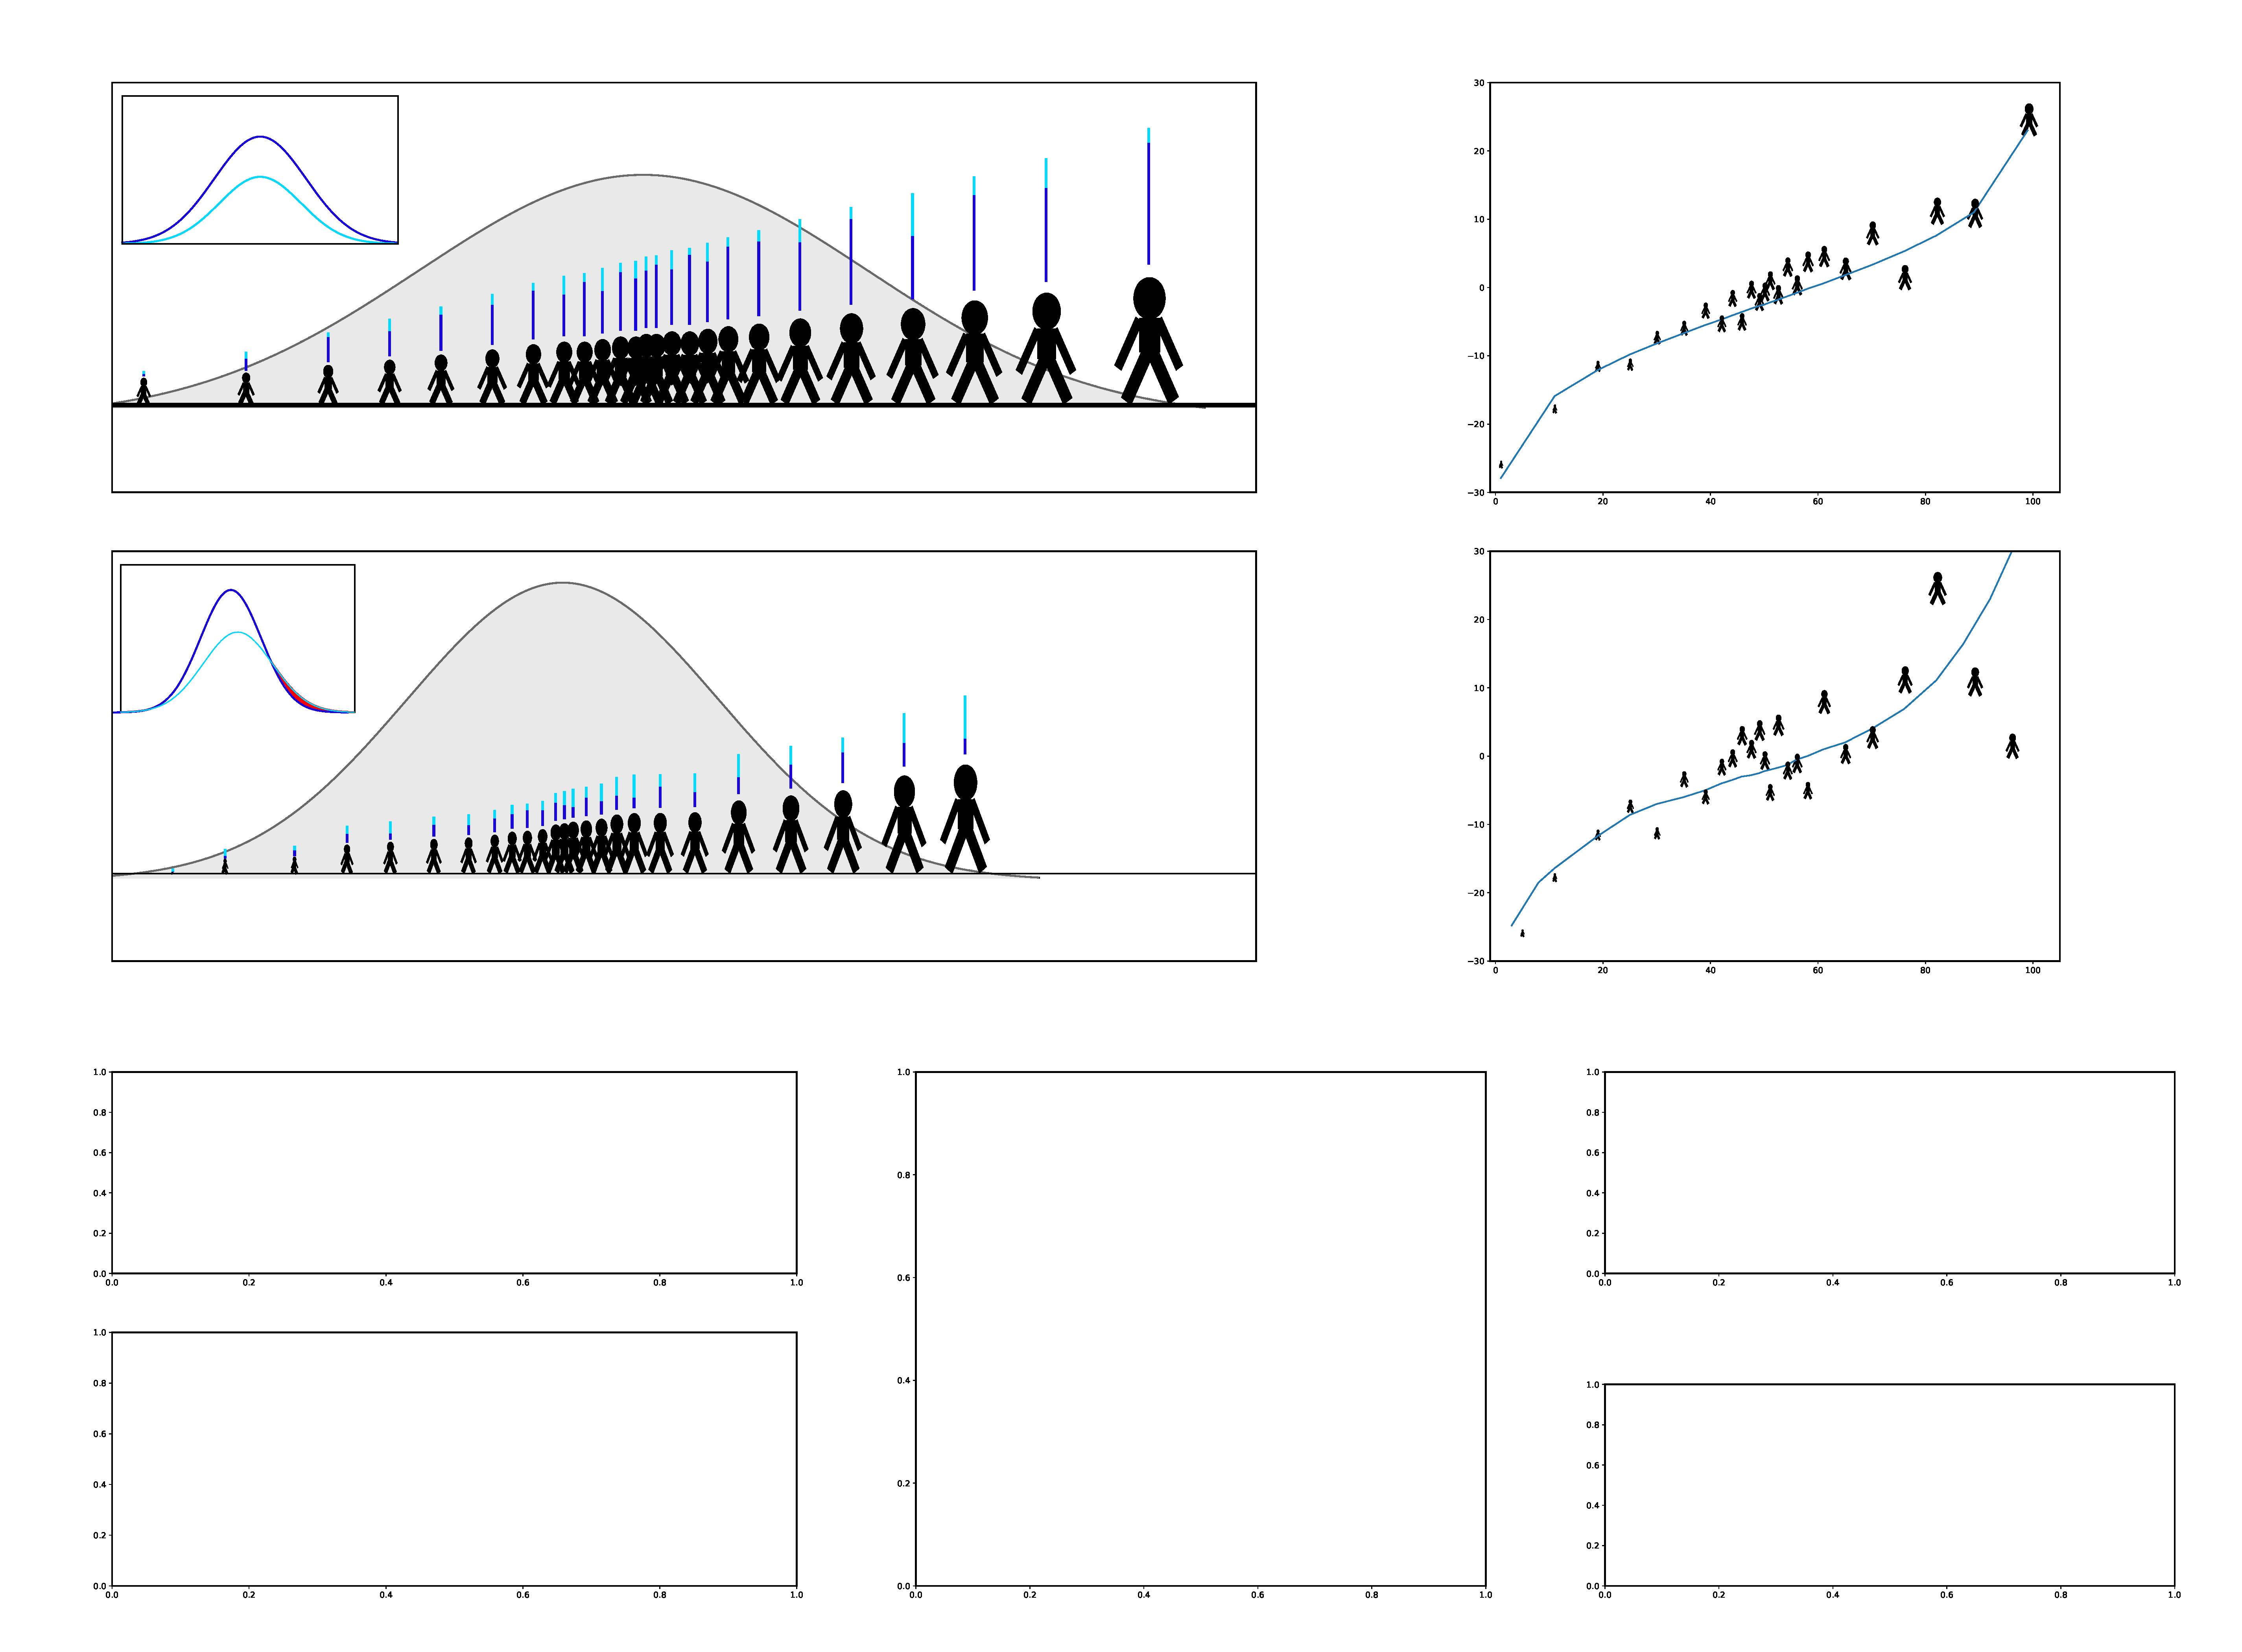
\includegraphics[trim=3cm 0cm 0cm 0cm, clip, width=1.2\textwidth]{Figures/Fig1.pdf}} \end{maybe} 
\caption{\footnotesize{\textbf{Model Schematic and Simulated Results}} 
\textbf{(d)} Simulated Result: Distribution after stabilising selection. 
\textbf{(e)} Simulated Result: Trumpet plot before and after stabilising selection.  
\textbf{(f)} Simulated Result: Contribution of rare variants across the distribution under stabilising selection. 
\textbf{(g)} Simulated Result: Trait quantile vs mean quantile calculated using all variants (top) and only variants with MAF>1\%.} 
\label{fig:sim} \end{figure} \FloatBarrier 



Motivated by \need{simulated results that demonstrating the relationship 
between selection, rare variants and POPout (see \fref{fig:sim})},  we selected UKB biobank traits 
for analyses from the following categories  
\textit{Biomarkers}, \textit{Physical Measures}, 
\textit{Touchscreen Questionnaire} and  \textit{Cognitive Tests}.  
Continuous traits from these categories were standardised by regressing 
out the effects of age, sex, and known environmental and technical factors 
and then applying an inverse-normal transformation (see \textit{Methods: Trait Normalisation}).  
Samples were then split in half, GWAS was carried out using Plink \cite{bt_10}, 
and heritability and pairwise genetic correlation was estimated using LDscore \cite{ldsc}.
Applying quality controls for sample size, heritability, skew, and oligogenicity and 
removing strongly correlated traits resulted in the set of 74 traits (see \textit{Methods: Trait QC}), 
used for the POPout associated analyses conducted across the large number of European ancestry 
samples in the UK Biobank and replicated three ways: 
across a subset of repeated measures European ancestry samples in the UK Biobank, 
acorss a subset of non-European ancestry samples in the UK Biobank, and, where applicable, 
across European ancestry samples in the All Of Us Biobank (see \textit{Replication}). 


\subsection*{The POPout Test} ~\\ 

Conceptually, POPout occurs when when samples in the tails of the trait phenotype 
distribution have polygenic scores that significantly depart from expectation.  
To quantify this phenomenon we have developed the \textit{POPout test} which regresses
PRS-On-Phenotype to estimate the effect size, direction, and significance of departure from expected PRS 
for individuals in the lower and upper 1\% of the trait distribution (see \textit{Methods}).  

Applying this test to the European ancestry samples in the UK-biobank reveals widespread departure 
from expectation across the 74 traits analysed.  Correcting for multiple tests (5\% false discovery threshold), 
68 of 74 traits have significant POPout effects in one or both tails and that the vast majority (90\%) of these 
effects are positive - i.e. reflect regression to the mean or unexpectedly mild risk scores - 
which is consistent with rare variants of large effects in individuals of the trait tails. 
\dref{fig:pop}{a} illustrates the three broad types of tail effects by plotting trait quantile, 
in 1\% increments, versus mean PRS in the quantile for four index traits: 
\begin{itemize} 
\item \textit{Phosphate} - Selected because it has no observable $POPout$ Effect in either tail.  
\item \textit{Haemoglobin Concentration} - selected for most significant POPout regression in lower tail only, 
\item \textit{Red Blood Cell Distribution Width} - selected for most significant POPout regression in upper tail only, 
\item \textit{Sitting Height} - selected for most significant POPout regression in both tails (minimum value).   
\end{itemize} 
        

\noindent \dref{fig:pop}{b} enumerates the POPout tail effects for all traits analyzed, separated into three logical UKB categories, \textit{Biomarkers}, \textit{Physical Measures} 
and \textit{Questionnaire/Cognitive}.  Again positive POPout effects (regression to the mean) predominate, especially with respect to larger effects: 22 tails have 
positive POPout effects greater than 0.25 while none have negative POPout effects less than 0.25.  Here we also observe that POPout regression is 
most common in \textit{Biomarkers} category (79\% of tails) and least common in \textit{Questionnaire/Cognitive} category (43\% of tails). Overall 
we observe a moderate relationship ($R=0.23,Pv=0.018$) between POPout regression and trait heritability, suggesting that POPout regression is 
not driven primarily by environmental effects.  

\dref{fig:pop}{c} illustrates the impact that tail $POPout$ has on the reliability of PRS model to predict phenotype in the upper tails.  
For both traits shown, \textit{Haemoglobin Concentration} and \textit{Red Blood Cell Distribution Width} the relative odds ratios are 
equal to expectation when "case" is defined very liberally - as being in lower or upper 25\% of the distribution but underperform in 
the presence of $POPout$ when "case" is defined conservatively - being in the lower or upper 1\% of the distribution.  
With respect to \textit{Haemoglobin Concentration}, where lower tail $POPout$ is present, the relative odds ratio for the lowest $PRS$ 
quantile ($5\%$) when case is defined as being in the lower 1\% is only 1.5, which is far below expectation and far below the 
upper tail analogue (top quantile ($95\%$ predicts case defined by upper 1\%) which is 3.5. 
With respect to \textit{Red Blood Cell Distribution Width}, where upper tail $POPout$ is present, the relative odds ratio for the largest $PRS$ 
quantile ($95\%$) when case is defined as being in the upper 1\% is only 1.7, which is far below expectation and far below the 
lower tail analogue (bottom quantile ($5\%$ predicts case defined by lower 1\%) which is 5.1. This shows that while the presence of 
$POPout$ in one or both tails does not preclude overall predictive power as defined using $PRS$ $r^2$ it can cause the $PRS$ to obtain 
all its predictive power by using the moderate range of the distribution, causing $PRS$ models to describe the genetic architecture that 
underlies a range of moderate phenotypes that excludes the extremes where disease is more likely to manifest. 


In figure \dref{fig:pop}{d} the results of three flavours of $POPout$ replication performed on $POPout$ effect sizes is shown. 
In each replication dataset, matching traits with at least five thousand samples that passed our \textit{$POPout$ regression QC} 
mentioned above were included and the Pearson correlation across the $POPout$ tail effect sizes was calculated. 



Replication across the mean in a small samples of repeated measures (50 traits, $R=0.71,Pvalue=2.3 \times 10^{-16}$) 
in UKB samples of European ancestry demonstrates that $POPout$ effects are unlikely to be caused by random measurement errors that drive individuals to the tails of the distribution. 
Replication in UKB-samples of Non-European ancestry (54 traits, $R=0.63,Pvalue=3.7 \times 10^{-13}$) 
demonstrate that $POPout$ is not an ancestry specific phenomenon. 
Lastly, replication in the $All of Us$ cohort (28 traits, $R=0.59,Pvalue=1.6 \times 10^{-6}$) 
demonstrate that $POPout$ is not a UKB specific phenomenon as a matched ancestry sample 
in a different country also has similar results. For more information on replication please see \textit{supplement}. 
Interestingly, the correlation across ancestry (UKB European and non-European) samples is higher than the 
within ancestry across biobank correlation (UKB European and All of Us European) which suggests that despite 
accurate PRS prediction not being portable across ancestry that POPout regression is still portable across ancestry groups. 



\clearpage \newpage 

\FloatBarrier \begin{figure}[!h] \centering \begin{maybe}{showFig} 
\centerline{\includegraphics[trim=0cm 0cm 0cm 0cm, clip, width=1.3\linewidth]{Figures/Fig2.pdf}} \end{maybe} 
\caption{\footnotesize{{\bf Tail POPout.} 
\textbf{(a)} PRS quantile (in 1\% increments) plotted against mean trait value for four traits with
different POP-out results (clockwise: No $POPout$ Effects, $POPout$ in Upper Tail, Lower Tail, Dual Tail). 
\textbf{(b)} POPout results for all 74 traits separated  by category. 
\textbf{(c)} Case Control Accuracy Test 
\textbf{(d)} Replication 
}} \label{fig:pop} \end{figure} \FloatBarrier


%In \fref{fig:rep}{a} trait quantile is plotted in 1\% increments versus mean PRS in the quantile of our index traits, with 
%\textit{Height} and \textit{Weight} subsituting for \textit{Phosphate} and \textit{Sitting Height} which are 
%not available in the the \textit{All Of Us} dataset.  Visual concordance can be observed across the European ancestry 
%repeated measures, the non-European samples and the \textit{All Of Us} dataset.  In \fref{fig:rep}{b} POPout effect 
%sizes and confidence intervals are shown for all traits avaialble across the biobanks.  In \fref{fig:rep}{c-e} the 
%significant correlations across averaged measures, non-European samples, and \textit{All Of Us} are shown.  Interestingly, 
%the correlation across ancestry (UKB European and non-European) samples is higher than the correlation across biobanks 
%but within ancestry which suggests that despite accurate PRS prediction not being portable across ancestry that 
%POPout regression is still portable across ancestry groups. 








%%%%%%%%%%%%%%%%%%%%%%%%%%%%%%%%%%%%%%%%%%%%%%%%%%%%%%%%%%%%%%%%%%%%%%%%
%%%%%%%%%%%%%%%%%%%%%%%%%%%%  FIGURE 3 %%%%%%%%%%%%%%%%%%%%%%%%%%%%%%%%%
%%%%%%%%%%%%%%%%%%%%%%%%%%%%%%%%%%%%%%%%%%%%%%%%%%%%%%%%%%%%%%%%%%%%%%%%

\clearpage \newpage
\subsection*{\emph{Replication in Siblings}} ~\\
Discordance between siblings in the tails of the trait distribution is
indictive non-polygenic inheritance \cite{avi}. Furthermore, excess
trait concordance between siblings can be indicative of shared
Mendelian effects \cite{t_sibs}. \fref{fig:sib}{a} illustartes the
expected impact of polygenicity, de novo, and Mendelian rare variants
within sibling pairs. Expected sibling pair concordance under
polygenicity can be used to test for (1) excess discordance between
siblings in tails of trait distribution, indicative of de novo
mutations of large in one sibling and (2) excess concordance between
siblings in tails of trait distribution, indicative of shared
Mendelian effects \cite{t_sibs}. These tests are derived from the
conditional sibling distribution under polygenicity, this distribution
also allows heritability to be estimated \cite{t_sibs}.

Applying this model to the sibling data in the UKB to estimate $h^2$, 
we find a correlation between snp h2 and sibling h2 in \fref{fig:sib}{b}.  
As shown in \fref{fig:sib}{c}, we use this model to infer the presence of rare variant 
architecture in our index traits and find lower tail discordance 
in \emph{Haemoglobin Concentration}, upper tail discordance in 
\emph{Red Blood Cell Distribution Width} and dual ail discordance 
in \emph{Sitting Height}, all of which match the result of the POPout analyses. 
We also find an overall significant relationship between sibling test pvalue and the POPout pvalue across all 74 traits \fref{fig:sib}{d}. 
Interestingly, this relationship varies across category, pearson correlation is $0.80$ across the \textit{Biomarker} group, 
$0.60$ across the \textit{Physical Measures} and insignificant the lower heritability \textit{Questionnaire/Cognitive} category suggesting again 
that concordance between POPout effects and sibling discordance is not the result environmental causes alone. 



%
\includegraphics[width=0.9\textwidth]{Figures/fig.eps}


\FloatBarrier \begin{figure}[!h] \begin{maybe}{showFig} 
\centerline{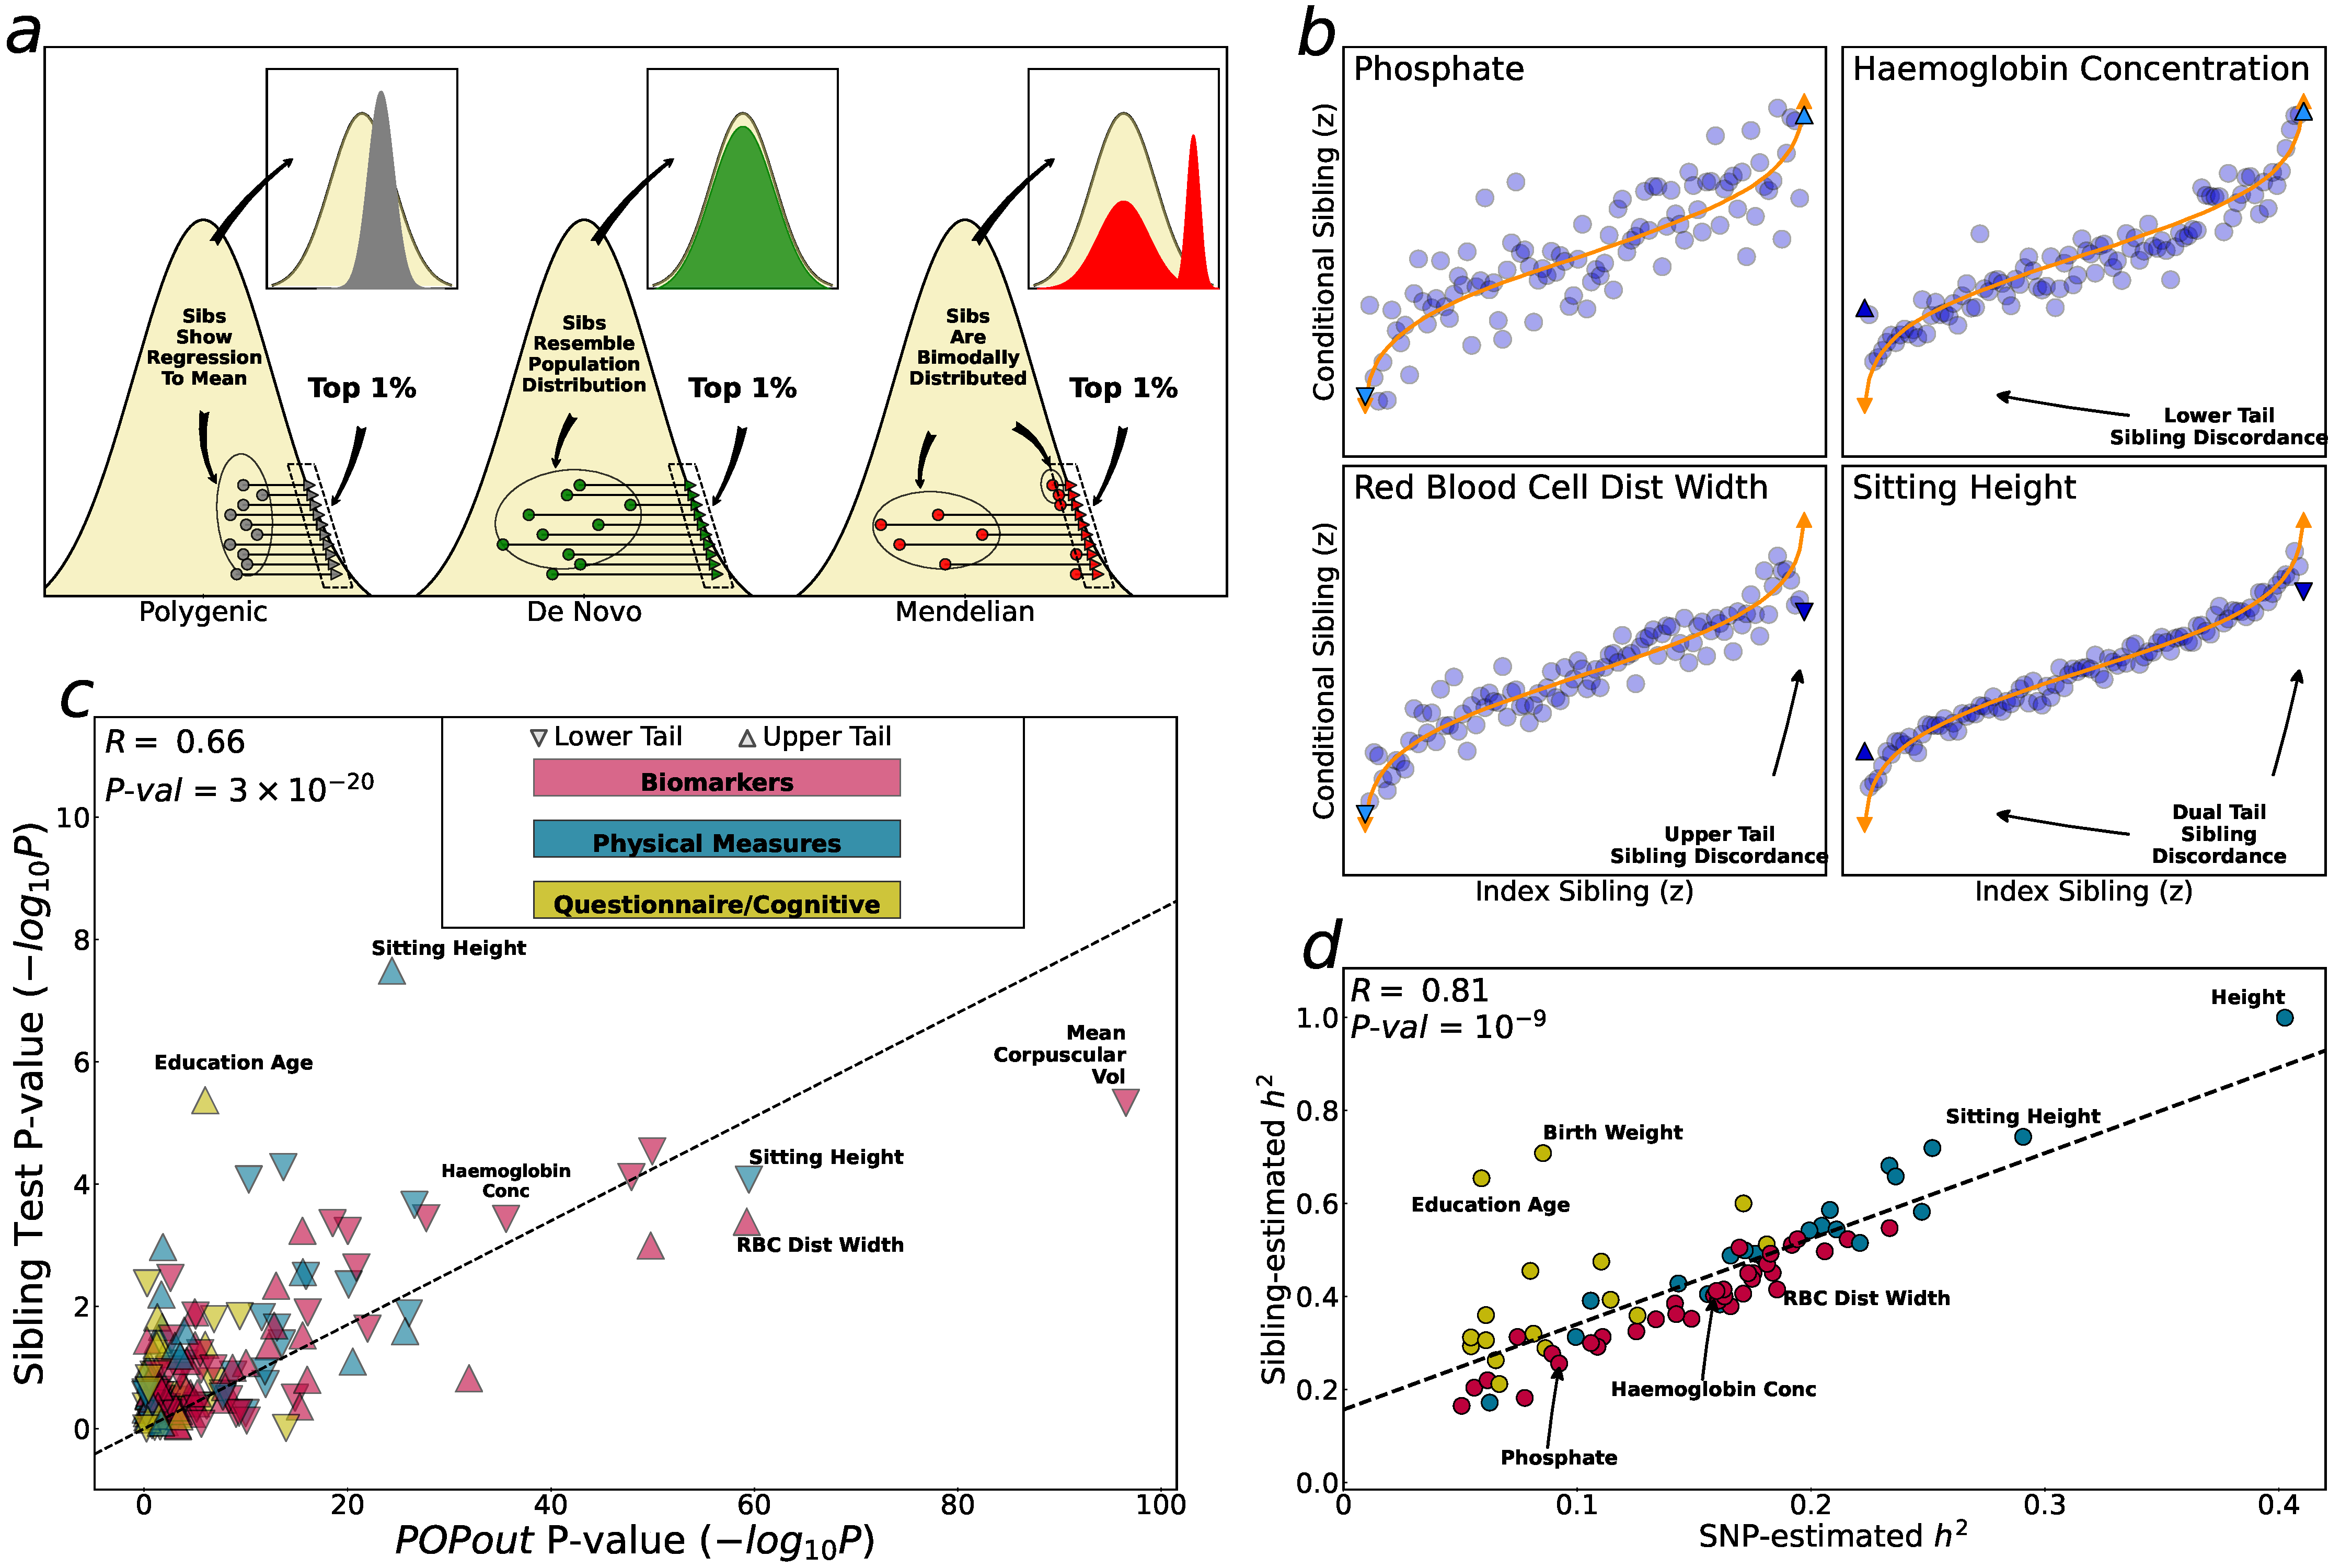
\includegraphics[trim=0cm 0cm 0cm 0cm, clip, width=1.2\linewidth]{Figures/Fig3.pdf}} \end{maybe} 
%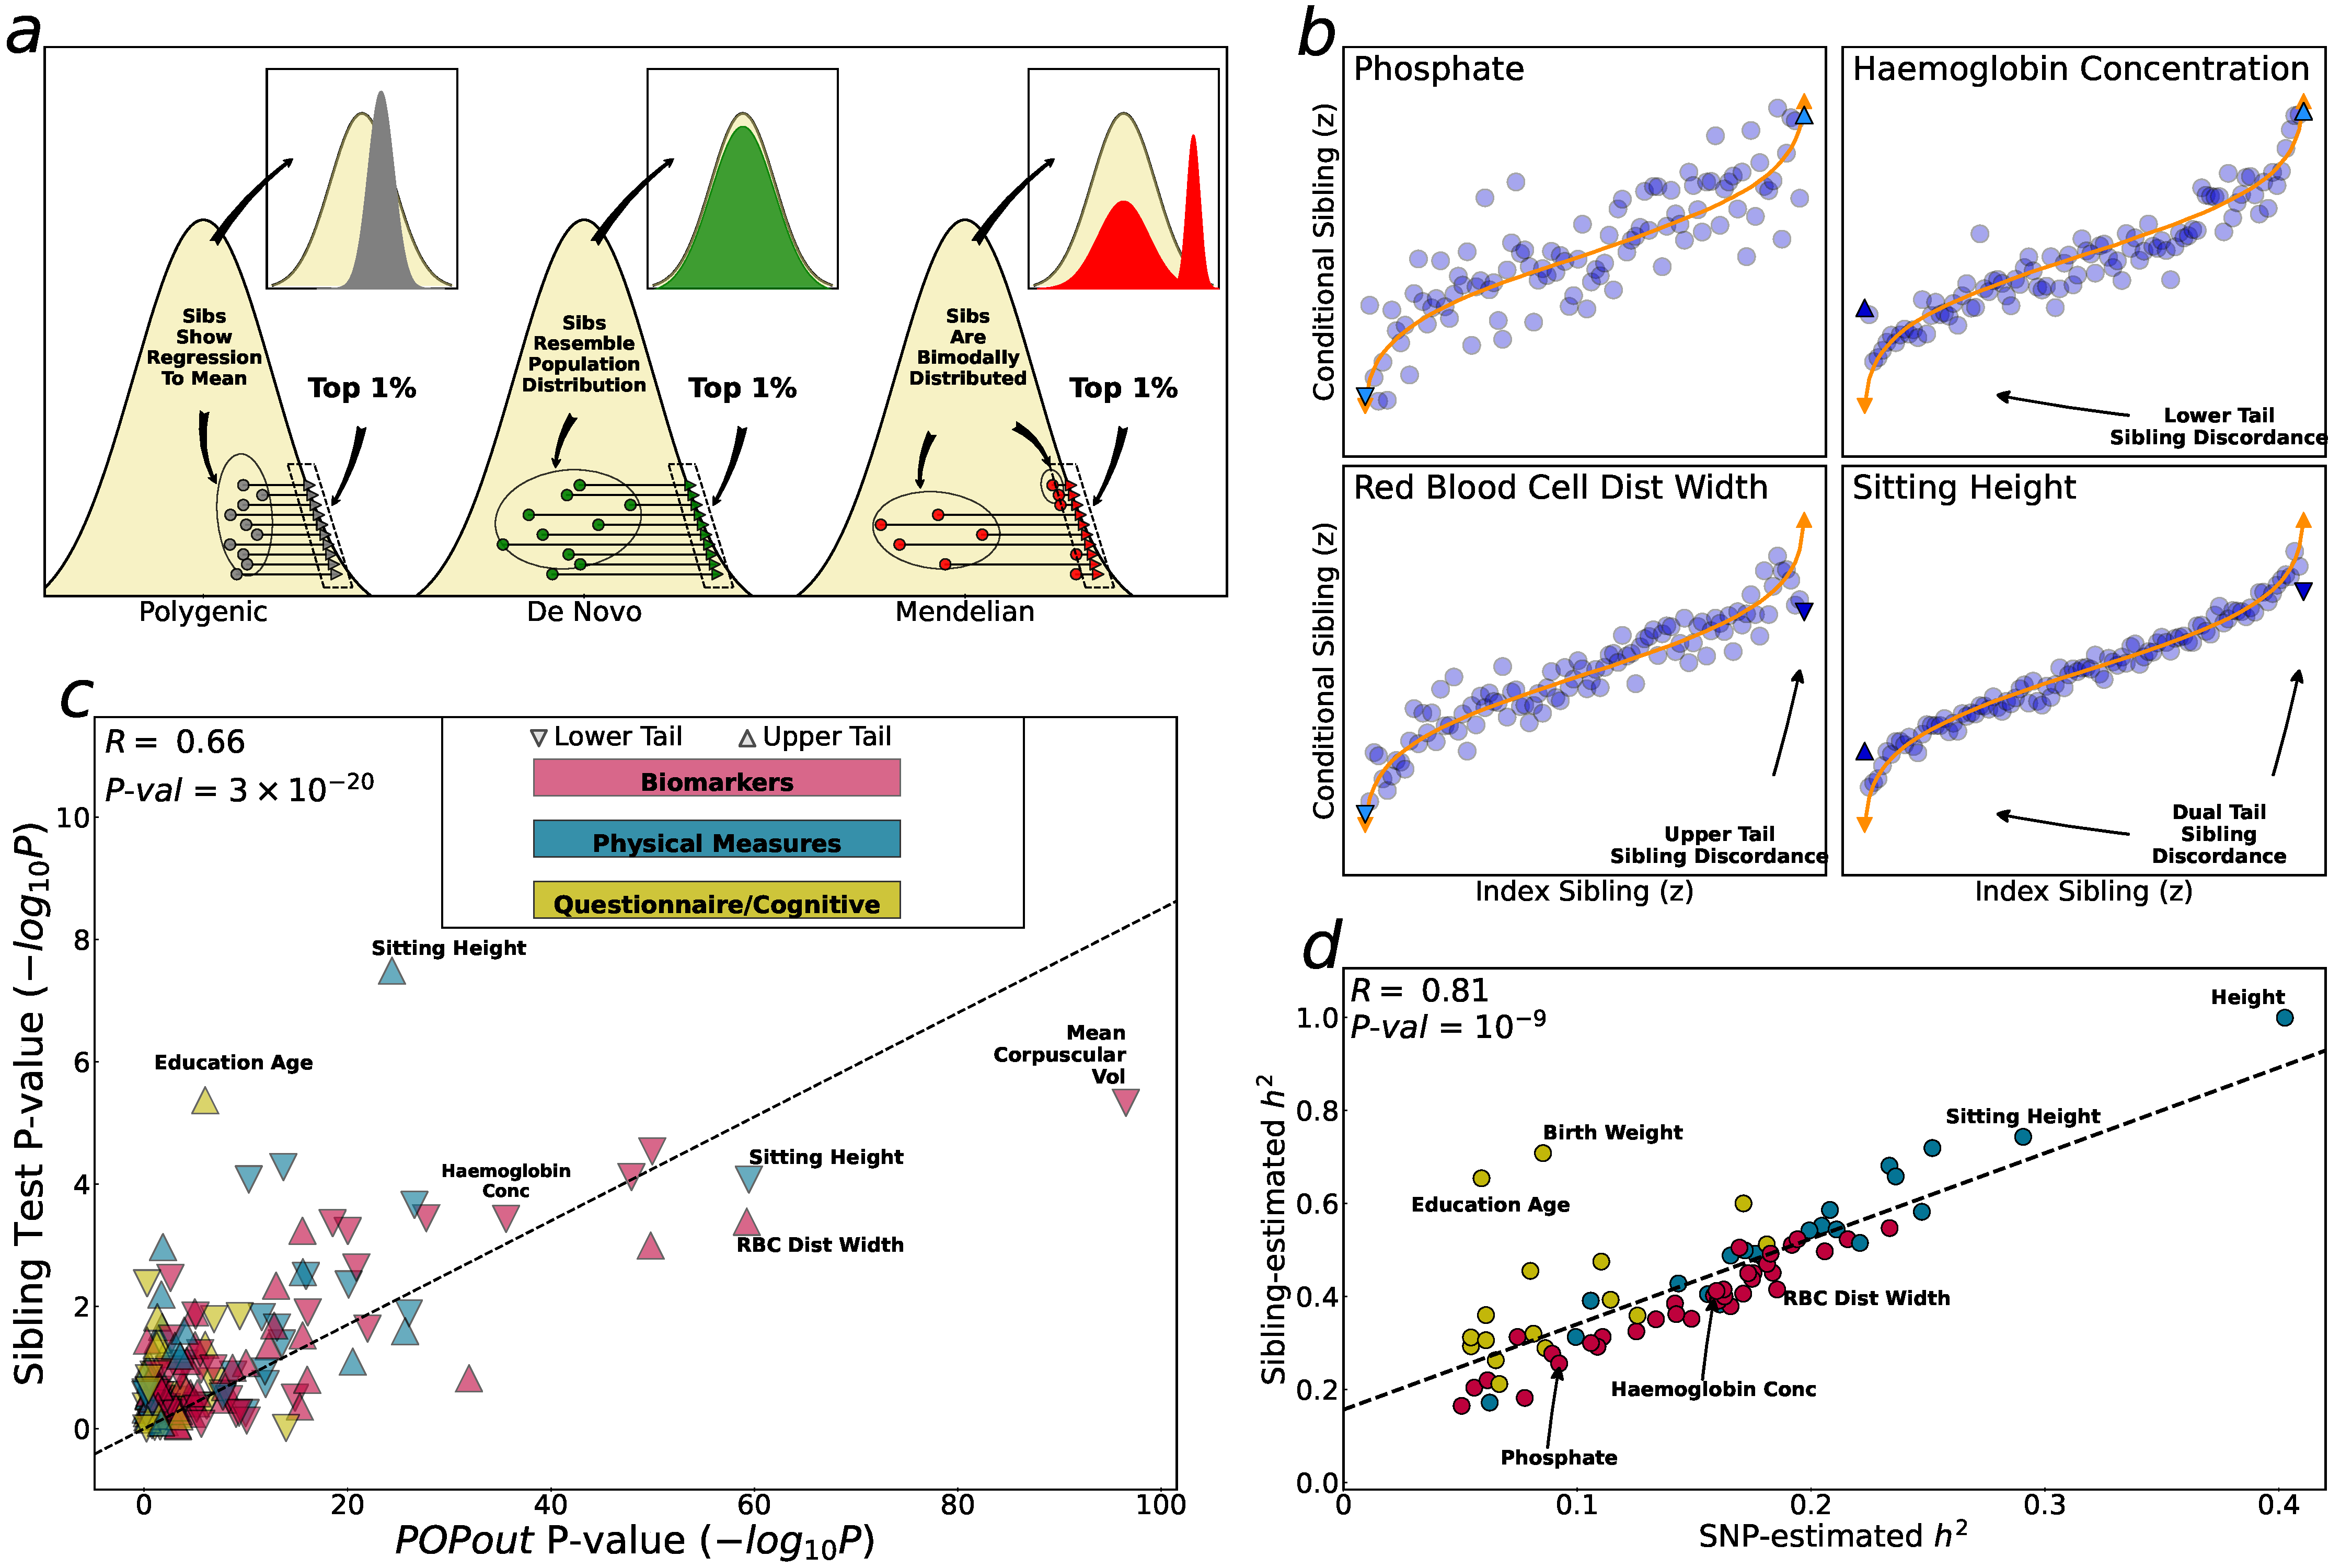
\includegraphics[trim=0cm 0cm 0cm 0cm, clip, width=\linewidth]{Figures/Fig3.pdf} \end{maybe} 
\caption{\footnotesize{{\bf $POPout$ Replication in Siblings.} 
\textbf{(a)} Schematic of relationship of sibling trait values
under polygenicity, de novo variants of large effect in one
sibling and rare inherited variant of large effect,
Mendelian. \textbf{(b)} LDscore regression SNP
heritability plotted against heritability estimated from sibling
pair trait similarity using European UKB samples.  \textbf{(c)}
Index sibling trait quantile (in 1\% increments) plotted agaisnt
mean trait value of conditional sibling in quantile for four
traits with different types of PRS tail regression. \textbf{(d)}
PRS-test P-values plotted against sibling de novo and Mendelian
test meta analysis P-values on $-\log_{10}$ scale for upper and
lower tails of all 74 traits.  Correlation calculated using
pearson correlation.}} 
\label{fig:sib} \end{figure} \FloatBarrier


\clearpage \newpage
%%%%%%%%%%%%%%%%%%%%%%%%%%%%%%%%%%%%%%%%%%%%%%%%%%%%%%%%%%%%%%%%%%%%%%%%
%%%%%%%%%%%%%%%%%%%%%%%%%%%%  FIGURE 4 %%%%%%%%%%%%%%%%%%%%%%%%%%%%%%%%%
%%%%%%%%%%%%%%%%%%%%%%%%%%%%%%%%%%%%%%%%%%%%%%%%%%%%%%%%%%%%%%%%%%%%%%%%

\subsection*{The Role of Rare Variants} ~\\

\FloatBarrier \begin{figure}[!h] 
\begin{maybe}{showFig}
\centerline{\includegraphics[trim=0cm 0cm 0cm 0cm, clip, width=1.2\linewidth]{Figures/Fig4.pdf}}
\end{maybe} 
\caption{\footnotesize{{\bf Rare Variant and Selection Analysis}} 
\textbf{(a)} Trumpet plots (minor allele frequency v effect size) of genome-wide significant variants for traits shown in (a). 
\textbf{(b)} POP-out effect sizes plotted against the number of genome-wide significant
variants with MAF<1\% for 58 traits with overlapping exome sequence results. 
For upper tails positive variant effects are counted and for lower tails negative variant effects are counted. 
Correlation and significance calculated using pearson correlation.
\textbf{(c)} Age at Menopause: PRS quantile vs. trait mean and trumpet plot.  
\textbf{(d)} Residualised trait value plotted against relative lifetime reproductive success for 16 example traits.
Best model fit to the data, selected by BIC considering all models with and without linear and quadratic terms, 
are shown by dashed lines. Model selected by BIC used to classify selective pressure acting on the traits. 
\textbf{(e)} $POPout$ effect size shown by model selection category, with PRS-test effect size meta-analysis for each category. 
\textbf{(f)} Spearman rank correlation between four proxy measures of fitness and PRS-test effect size. For each 
fitness measure correlation was calculated between the mean of the fitness measure in individuals in the upper and lower 1\% tails
and PRS-test effect size for the corresponding tail across 74 traits in UKB passing QC.}
\label{fig:evo} \end{figure} \FloatBarrier






\noindent The genetic mechanism proposed to explain $POPout$ involves the confluence 
of genetic selection away from one or both tails, an enrichment of rare variants in those tails, 
and PRS methods that typically restrict to common variants (MAF $>1\%$) that suffers in such tails.  
Indeed, the exclusion of rare variants from PRS has already been shown to 
reduce PRS performance \citep{rares1}. \fref{fig:evo}{a} shows
the relationship between MAF and effect sizes from significant
associations derived from GWAS \citep{neale} and exome analyses
\citep{backman} of UKB for our four index traits. For \textit{Haemoglobin
Concentration} which exhibits lower tail regression we see a greater
number of rare variants in the lower tail and for \textit{Red Blood Cell
Distribution Width} which exhibits upper tail regression we see a
greater number of rare variants in the upper tail. Sitting height,
which exhibits dual tail regression, has a number of rare variants in
both tails, however, there are more rare variants in the lower tail
where the POPout effect is greatest. For \textit{Phosphate} which does
not exhibit POPout in either tail there are much fewer rare
variants of large effect.  These results are consistent with the hypothesis that
rare variants of large effect that not accounted for in the
common-variant PRS are responsible for tail POPout effects. 

Indeed this relationship holds up across all traits analysed.  In 
In \fref{fig:evo}{b} we observe a small but significant relationship
between the magnitude of \textit{POPOut} regression in the tail and the number of rare
variants in the tail across all trait tails analysed. However, we note that 
while statistically significant, there are multiple traits with significant 
\textit{POPout} scores for which almost no rare variants of substantially large effect 
have been identified (see \fref{fig:evo}{c}).  This suggests that strong selection 
may result in private variants that cannot be identified using population based sequencing.















\subsection*{The Impact of Selection} ~\\
Using adjusted lifetime reproductive success \citep{v_select, v_select2} as a proxy for selection 
we classified the selective pressure acting on each trait (see \textit{Methods} - LRS) by fitting it an 
optimal two parameter model ($Y_{LRS} = x_o+ \beta x + \gamma X^2$) as determined by BIC.  Shown 
in \fref{fig:evo}{a}, most traits (65 of 74\%) have some relationship (ie. $\beta \neq 0$ or $\gamma \neq 0$) 
between between adjusted lifetime success and trait quantile and the majority of them (43 of 65) 
two thirds of traits (43 of 65) were classified as being under some form of stabilising ($\gamma < 0$) selection, which is 
characterized by lower fecundity in the both tails of the trait distribution.  
This may be the result of general fitness  favoring the trait mean or the result of sex specific selection 
that averages to produce this relationship \citep{v_select}.  Only two traits were classified as under disruptive 
selection ($\gamma > 0$) which is characterised by greater fecundity in both trait tails. 

Irrespective of their gamma parameter, 57 trait models included a nonzero directional beta parameter.  
In \fref{fig:evo}{b} we see that traits under positive selection have significantly more POPout regression 
in the lower tail and that traits under negative selection have signficicantly more POPout regression 
in the positive tail - which is in line with theoretical and simulated predictions that suggest that 
negative selection drives an enrichment of rare variants in the tail which reducing polygenicity and 
driveout POPout regression.  



\subsubsection*{Tail Fitness} ~\\ 

In addition to model selection on adjusted lifetime reproductive sucess we analysed the 
relationship between five ranked fitness related measures associated with \emph{de novo} etiology 
and ranked POPout regression across all 148 tails analysed.  Shown in \fref{fig:evo}{c}, we find that 
while POPout regression is associated with less less offspring in both sexes, that this effect may 
be stronger in males.  Additionally we find that while neither the number of illnesses or miscarriages and 
stillbirths are significantly associated with POPout regression that paternal age \cite{pat} 
further suggesting that private variants may be driving some of the POPout signal. 












































%%%%%%%%%%%%%%%%%%%%%%%%%%%%%%%%%%%%%%%%%%%%%%%%%%%%%%%%%%%%%%%%%%%%%%%%%%%%%%%%%%%%
%%%%%%%%%%%%%%%%%%%%%%%%%%%%%%%%%%%%   END RESULTS %%%%%%%%%%%%%%%%%%%%%%%%%%%%%%%%%
%%%%%%%%%%%%%%%%%%%%%%%%%%%%%%%%%%%%%%%%%%%%%%%%%%%%%%%%%%%%%%%%%%%%%%%%%%%%%%%%%%%%
%
%
%
%
%
%
%
%
%
%
%
%
%
%
%




















\section{This is an example for first level head---section head}\label{sec3}

\subsection{This is an example for second level head---subsection head}\label{subsec2}

\subsubsection{This is an example for third level head---subsubsection head}\label{subsubsec2}

Sample body text. Sample body text. Sample body text. Sample body text. Sample body text. Sample body text. Sample body text. Sample body text. 

\section{Equations}\label{sec4}

Equations in \LaTeX\ can either be inline or on-a-line by itself (``display equations''). For
inline equations use the \verb+$...$+ commands. E.g.: The equation
$H\psi = E \psi$ is written via the command \verb+$H \psi = E \psi$+.

For display equations (with auto generated equation numbers)
one can use the equation or align environments:
\begin{equation}
\|\tilde{X}(k)\|^2 \leq\frac{\sum\limits_{i=1}^{p}\left\|\tilde{Y}_i(k)\right\|^2+\sum\limits_{j=1}^{q}\left\|\tilde{Z}_j(k)\right\|^2 }{p+q}.\label{eq1}
\end{equation}
where,
\begin{align}
D_\mu &=  \partial_\mu - ig \frac{\lambda^a}{2} A^a_\mu \nonumber \\
F^a_{\mu\nu} &= \partial_\mu A^a_\nu - \partial_\nu A^a_\mu + g f^{abc} A^b_\mu A^a_\nu \label{eq2}
\end{align}
Notice the use of \verb+\nonumber+ in the align environment at the end
of each line, except the last, so as not to produce equation numbers on
lines where no equation numbers are required. The \verb+\label{}+ command
should only be used at the last line of an align environment where
\verb+\nonumber+ is not used.
\begin{equation}
Y_\infty = \left( \frac{m}{\textrm{GeV}} \right)^{-3}
    \left[ 1 + \frac{3 \ln(m/\textrm{GeV})}{15}
    + \frac{\ln(c_2/5)}{15} \right]
\end{equation}
The class file also supports the use of \verb+\mathbb{}+, \verb+\mathscr{}+ and
\verb+\mathcal{}+ commands. As such \verb+\mathbb{R}+, \verb+\mathscr{R}+
and \verb+\mathcal{R}+ produces $\mathbb{R}$, $\mathscr{R}$ and $\mathcal{R}$
respectively (refer Subsubsection~\ref{subsubsec2}).

\section{Tables}\label{sec5}

Tables can be inserted via the normal table and tabular environment. To put
footnotes inside tables you should use \verb+\footnotetext[]{...}+ tag.
The footnote appears just below the table itself (refer Tables~\ref{tab1} and \ref{tab2}). 
For the corresponding footnotemark use \verb+\footnotemark[...]+

\begin{table}[h]
\caption{Caption text}\label{tab1}%
\begin{tabular}{@{}llll@{}}
\toprule
Column 1 & Column 2  & Column 3 & Column 4\\
\midrule
row 1    & data 1   & data 2  & data 3  \\
row 2    & data 4   & data 5\footnotemark[1]  & data 6  \\
row 3    & data 7   & data 8  & data 9\footnotemark[2]  \\
\botrule
\end{tabular}
\footnotetext{Source: This is an example of table footnote. This is an example of table footnote.}
\footnotetext[1]{Example for a first table footnote. This is an example of table footnote.}
\footnotetext[2]{Example for a second table footnote. This is an example of table footnote.}
\end{table}

\noindent
The input format for the above table is as follows:

%%=============================================%%
%% For presentation purpose, we have included  %%
%% \bigskip command. Please ignore this.       %%
%%=============================================%%
\bigskip
\begin{verbatim}
\begin{table}[<placement-specifier>]
\caption{<table-caption>}\label{<table-label>}%
\begin{tabular}{@{}llll@{}}
\toprule
Column 1 & Column 2 & Column 3 & Column 4\\
\midrule
row 1 & data 1 & data 2	 & data 3 \\
row 2 & data 4 & data 5\footnotemark[1] & data 6 \\
row 3 & data 7 & data 8	 & data 9\footnotemark[2]\\
\botrule
\end{tabular}
\footnotetext{Source: This is an example of table footnote. 
This is an example of table footnote.}
\footnotetext[1]{Example for a first table footnote.
This is an example of table footnote.}
\footnotetext[2]{Example for a second table footnote. 
This is an example of table footnote.}
\end{table}
\end{verbatim}
\bigskip
%%=============================================%%
%% For presentation purpose, we have included  %%
%% \bigskip command. Please ignore this.       %%
%%=============================================%%

\begin{table}[h]
\caption{Example of a lengthy table which is set to full textwidth}\label{tab2}
\begin{tabular*}{\textwidth}{@{\extracolsep\fill}lcccccc}
\toprule%
& \multicolumn{3}{@{}c@{}}{Element 1\footnotemark[1]} & \multicolumn{3}{@{}c@{}}{Element 2\footnotemark[2]} \\\cmidrule{2-4}\cmidrule{5-7}%
Project & Energy & $\sigma_{calc}$ & $\sigma_{expt}$ & Energy & $\sigma_{calc}$ & $\sigma_{expt}$ \\
\midrule
Element 3  & 990 A & 1168 & $1547\pm12$ & 780 A & 1166 & $1239\pm100$\\
Element 4  & 500 A & 961  & $922\pm10$  & 900 A & 1268 & $1092\pm40$\\
\botrule
\end{tabular*}
\footnotetext{Note: This is an example of table footnote. This is an example of table footnote this is an example of table footnote this is an example of~table footnote this is an example of table footnote.}
\footnotetext[1]{Example for a first table footnote.}
\footnotetext[2]{Example for a second table footnote.}
\end{table}

In case of double column layout, tables which do not fit in single column width should be set to full text width. For this, you need to use \verb+\begin{table*}+ \verb+...+ \verb+\end{table*}+ instead of \verb+\begin{table}+ \verb+...+ \verb+\end{table}+ environment. Lengthy tables which do not fit in textwidth should be set as rotated table. For this, you need to use \verb+\begin{sidewaystable}+ \verb+...+ \verb+\end{sidewaystable}+ instead of \verb+\begin{table*}+ \verb+...+ \verb+\end{table*}+ environment. This environment puts tables rotated to single column width. For tables rotated to double column width, use \verb+\begin{sidewaystable*}+ \verb+...+ \verb+\end{sidewaystable*}+.

\begin{sidewaystable}
\caption{Tables which are too long to fit, should be written using the ``sidewaystable'' environment as shown here}\label{tab3}
\begin{tabular*}{\textheight}{@{\extracolsep\fill}lcccccc}
\toprule%
& \multicolumn{3}{@{}c@{}}{Element 1\footnotemark[1]}& \multicolumn{3}{@{}c@{}}{Element\footnotemark[2]} \\\cmidrule{2-4}\cmidrule{5-7}%
Projectile & Energy	& $\sigma_{calc}$ & $\sigma_{expt}$ & Energy & $\sigma_{calc}$ & $\sigma_{expt}$ \\
\midrule
Element 3 & 990 A & 1168 & $1547\pm12$ & 780 A & 1166 & $1239\pm100$ \\
Element 4 & 500 A & 961  & $922\pm10$  & 900 A & 1268 & $1092\pm40$ \\
Element 5 & 990 A & 1168 & $1547\pm12$ & 780 A & 1166 & $1239\pm100$ \\
Element 6 & 500 A & 961  & $922\pm10$  & 900 A & 1268 & $1092\pm40$ \\
\botrule
\end{tabular*}
\footnotetext{Note: This is an example of table footnote this is an example of table footnote this is an example of table footnote this is an example of~table footnote this is an example of table footnote.}
\footnotetext[1]{This is an example of table footnote.}
\end{sidewaystable}

\section{Figures}\label{sec6}

As per the \LaTeX\ standards you need to use eps images for \LaTeX\ compilation and \verb+pdf/jpg/png+ images for \verb+PDFLaTeX+ compilation. This is one of the major difference between \LaTeX\ and \verb+PDFLaTeX+. Each image should be from a single input .eps/vector image file. Avoid using subfigures. The command for inserting images for \LaTeX\ and \verb+PDFLaTeX+ can be generalized. The package used to insert images in \verb+LaTeX/PDFLaTeX+ is the graphicx package. Figures can be inserted via the normal figure environment as shown in the below example:

%%=============================================%%
%% For presentation purpose, we have included  %%
%% \bigskip command. Please ignore this.       %%
%%=============================================%%
\bigskip
\begin{verbatim}
\begin{figure}[<placement-specifier>]
\centering
\includegraphics{<eps-file>}
\caption{<figure-caption>}\label{<figure-label>}
\end{figure}
\end{verbatim}
\bigskip
%%=============================================%%
%% For presentation purpose, we have included  %%
%% \bigskip command. Please ignore this.       %%
%%=============================================%%

\begin{figure}[h]
\centering

\includegraphics[width=0.9\textwidth]{Figures/fig.eps}
\caption{This is a widefig. This is an example of long caption this is an example of long caption  this is an example of long caption this is an example of long caption}\label{fig1}
\end{figure}

In case of double column layout, the above format puts figure captions/images to single column width. To get spanned images, we need to provide \verb+\begin{figure*}+ \verb+...+ \verb+\end{figure*}+.

For sample purpose, we have included the width of images in the optional argument of \verb+\includegraphics+ tag. Please ignore this. 

\section{Algorithms, Program codes and Listings}\label{sec7}

Packages \verb+algorithm+, \verb+algorithmicx+ and \verb+algpseudocode+ are used for setting algorithms in \LaTeX\ using the format:

%%=============================================%%
%% For presentation purpose, we have included  %%
%% \bigskip command. Please ignore this.       %%
%%=============================================%%
\bigskip
\begin{verbatim}
\begin{algorithm}
\caption{<alg-caption>}\label{<alg-label>}
\begin{algorithmic}[1]
. . .
\end{algorithmic}
\end{algorithm}
\end{verbatim}
\bigskip
%%=============================================%%
%% For presentation purpose, we have included  %%
%% \bigskip command. Please ignore this.       %%
%%=============================================%%

You may refer above listed package documentations for more details before setting \verb+algorithm+ environment. For program codes, the ``verbatim'' package is required and the command to be used is \verb+\begin{verbatim}+ \verb+...+ \verb+\end{verbatim}+. 

Similarly, for \verb+listings+, use the \verb+listings+ package. \verb+\begin{lstlisting}+ \verb+...+ \verb+\end{lstlisting}+ is used to set environments similar to \verb+verbatim+ environment. Refer to the \verb+lstlisting+ package documentation for more details.

A fast exponentiation procedure:

\lstset{texcl=true,basicstyle=\small\sf,commentstyle=\small\rm,mathescape=true,escapeinside={(*}{*)}}
\begin{lstlisting}
begin
  for $i:=1$ to $10$ step $1$ do
      expt($2,i$);  
      newline() od                (*\textrm{Comments will be set flush to the right margin}*)
where
proc expt($x,n$) $\equiv$
  $z:=1$;
  do if $n=0$ then exit fi;
     do if odd($n$) then exit fi;                 
        comment: (*\textrm{This is a comment statement;}*)
        $n:=n/2$; $x:=x*x$ od;
     { $n>0$ };
     $n:=n-1$; $z:=z*x$ od;
  print($z$). 
end
\end{lstlisting}

\begin{algorithm}
\caption{Calculate $y = x^n$}\label{algo1}
\begin{algorithmic}[1]
\Require $n \geq 0 \vee x \neq 0$
\Ensure $y = x^n$ 
\State $y \Leftarrow 1$
\If{$n < 0$}\label{algln2}
        \State $X \Leftarrow 1 / x$
        \State $N \Leftarrow -n$
\Else
        \State $X \Leftarrow x$
        \State $N \Leftarrow n$
\EndIf
\While{$N \neq 0$}
        \If{$N$ is even}
            \State $X \Leftarrow X \times X$
            \State $N \Leftarrow N / 2$
        \Else[$N$ is odd]
            \State $y \Leftarrow y \times X$
            \State $N \Leftarrow N - 1$
        \EndIf
\EndWhile
\end{algorithmic}
\end{algorithm}

%%=============================================%%
%% For presentation purpose, we have included  %%
%% \bigskip command. Please ignore this.       %%
%%=============================================%%
\bigskip
\begin{minipage}{\hsize}%
\lstset{frame=single,framexleftmargin=-1pt,framexrightmargin=-17pt,framesep=12pt,linewidth=0.98\textwidth,language=pascal}% Set your language (you can change the language for each code-block optionally)
%%% Start your code-block
\begin{lstlisting}
for i:=maxint to 0 do
begin
{ do nothing }
end;
Write('Case insensitive ');
Write('Pascal keywords.');
\end{lstlisting}
\end{minipage}

\section{Cross referencing}\label{sec8}

Environments such as figure, table, equation and align can have a label
declared via the \verb+\label{#label}+ command. For figures and table
environments use the \verb+\label{}+ command inside or just
below the \verb+\caption{}+ command. You can then use the
\verb+\ref{#label}+ command to cross-reference them. As an example, consider
the label declared for Figure~\ref{fig1} which is
\verb+\label{fig1}+. To cross-reference it, use the command 
\verb+Figure \ref{fig1}+, for which it comes up as
``Figure~\ref{fig1}''. 

To reference line numbers in an algorithm, consider the label declared for the line number 2 of Algorithm~\ref{algo1} is \verb+\label{algln2}+. To cross-reference it, use the command \verb+\ref{algln2}+ for which it comes up as line~\ref{algln2} of Algorithm~\ref{algo1}.

\subsection{Details on reference citations}\label{subsec7}

Standard \LaTeX\ permits only numerical citations. To support both numerical and author-year citations this template uses \verb+natbib+ \LaTeX\ package. For style guidance please refer to the template user manual.

Here is an example for \verb+\cite{...}+: \cite{bib1}. %Another example for \verb+\citep{...}+: \citep{bib2}. For author-year citation mode, \verb+\cite{...}+ prints Jones et al. (1990) and \verb+\citep{...}+ prints (Jones et al., 1990).

All cited bib entries are printed at the end of this article: \cite{bib3}, \cite{bib4}, \cite{bib5}, \cite{bib6}, \cite{bib7}, \cite{bib8}, \cite{bib9}, \cite{bib10}, \cite{bib11}, \cite{bib12} and \cite{bib13}.


\section{Examples for theorem like environments}\label{sec10}

For theorem like environments, we require \verb+amsthm+ package. There are three types of predefined theorem styles exists---\verb+thmstyleone+, \verb+thmstyletwo+ and \verb+thmstylethree+ 

%%=============================================%%
%% For presentation purpose, we have included  %%
%% \bigskip command. Please ignore this.       %%
%%=============================================%%
\bigskip
\begin{tabular}{|l|p{19pc}|}
\hline
\verb+thmstyleone+ & Numbered, theorem head in bold font and theorem text in italic style \\\hline
\verb+thmstyletwo+ & Numbered, theorem head in roman font and theorem text in italic style \\\hline
\verb+thmstylethree+ & Numbered, theorem head in bold font and theorem text in roman style \\\hline
\end{tabular}
\bigskip
%%=============================================%%
%% For presentation purpose, we have included  %%
%% \bigskip command. Please ignore this.       %%
%%=============================================%%

For mathematics journals, theorem styles can be included as shown in the following examples:

\begin{theorem}[Theorem subhead]\label{thm1}
Example theorem text. Example theorem text. Example theorem text. Example theorem text. Example theorem text. 
Example theorem text. Example theorem text. Example theorem text. Example theorem text. Example theorem text. 
Example theorem text. 
\end{theorem}

Sample body text. Sample body text. Sample body text. Sample body text. Sample body text. Sample body text. Sample body text. Sample body text.

\begin{proposition}
Example proposition text. Example proposition text. Example proposition text. Example proposition text. Example proposition text. 
Example proposition text. Example proposition text. Example proposition text. Example proposition text. Example proposition text. 
\end{proposition}

Sample body text. Sample body text. Sample body text. Sample body text. Sample body text. Sample body text. Sample body text. Sample body text.

\begin{example}
Phasellus adipiscing semper elit. Proin fermentum massa
ac quam. Sed diam turpis, molestie vitae, placerat a, molestie nec, leo. Maecenas lacinia. Nam ipsum ligula, eleifend
at, accumsan nec, suscipit a, ipsum. Morbi blandit ligula feugiat magna. Nunc eleifend consequat lorem. 
\end{example}

Sample body text. Sample body text. Sample body text. Sample body text. Sample body text. Sample body text. Sample body text. Sample body text.

\begin{remark}
Phasellus adipiscing semper elit. Proin fermentum massa
ac quam. Sed diam turpis, molestie vitae, placerat a, molestie nec, leo. Maecenas lacinia. Nam ipsum ligula, eleifend
at, accumsan nec, suscipit a, ipsum. Morbi blandit ligula feugiat magna. Nunc eleifend consequat lorem. 
\end{remark}

Sample body text. Sample body text. Sample body text. Sample body text. Sample body text. Sample body text. Sample body text. Sample body text.

\begin{definition}[Definition sub head]
Example definition text. Example definition text. Example definition text. Example definition text. Example definition text. Example definition text. Example definition text. Example definition text. 
\end{definition}

Additionally a predefined ``proof'' environment is available: \verb+\begin{proof}+ \verb+...+ \verb+\end{proof}+. This prints a ``Proof'' head in italic font style and the ``body text'' in roman font style with an open square at the end of each proof environment. 

\begin{proof}
Example for proof text. Example for proof text. Example for proof text. Example for proof text. Example for proof text. Example for proof text. Example for proof text. Example for proof text. Example for proof text. Example for proof text. 
\end{proof}

Sample body text. Sample body text. Sample body text. Sample body text. Sample body text. Sample body text. Sample body text. Sample body text.

\begin{proof}[Proof of Theorem~{\upshape\ref{thm1}}]
Example for proof text. Example for proof text. Example for proof text. Example for proof text. Example for proof text. Example for proof text. Example for proof text. Example for proof text. Example for proof text. Example for proof text. 
\end{proof}

\noindent
For a quote environment, use \verb+\begin{quote}...\end{quote}+
\begin{quote}
Quoted text example. Aliquam porttitor quam a lacus. Praesent vel arcu ut tortor cursus volutpat. In vitae pede quis diam bibendum placerat. Fusce elementum
convallis neque. Sed dolor orci, scelerisque ac, dapibus nec, ultricies ut, mi. Duis nec dui quis leo sagittis commodo.
\end{quote}

Sample body text. Sample body text. Sample body text. Sample body text. Sample body text (refer Figure~\ref{fig1}). Sample body text. Sample body text. Sample body text (refer Table~\ref{tab3}). 







\section{Methods}\label{sec11}

Topical subheadings are allowed. Authors must ensure that their Methods section includes adequate experimental and characterization data necessary for others in the field to reproduce their work. Authors are encouraged to include RIIDs where appropriate. 

\textbf{Ethical approval declarations} (only required where applicable) Any article reporting experiment/s carried out on (i)~live vertebrate (or higher invertebrates), (ii)~humans or (iii)~human samples must include an unambiguous statement within the methods section that meets the following requirements: 

\begin{enumerate}[1.]
\item Approval: a statement which confirms that all experimental protocols were approved by a named institutional and/or licensing committee. Please identify the approving body in the methods section

\item Accordance: a statement explicitly saying that the methods were carried out in accordance with the relevant guidelines and regulations

\item Informed consent (for experiments involving humans or human tissue samples): include a statement confirming that informed consent was obtained from all participants and/or their legal guardian/s
\end{enumerate}

If your manuscript includes potentially identifying patient/participant information, or if it describes human transplantation research, or if it reports results of a clinical trial then  additional information will be required. Please visit (\url{https://www.nature.com/nature-research/editorial-policies}) for Nature Portfolio journals, (\url{https://www.springer.com/gp/authors-editors/journal-author/journal-author-helpdesk/publishing-ethics/14214}) for Springer Nature journals, or (\url{https://www.biomedcentral.com/getpublished/editorial-policies\#ethics+and+consent}) for BMC.



\subsection*{Data Processing} ~\\
\vspace*{-0.3cm} 
\subsubsection*{UK Biobank Genetic Data} ~\\
The UK Biobank (UKB) is a prospective cohort study of approximately
500,000 participants recruited across the United Kingdom from 2006 to
2010 \citep{ukb}. Phenotype data of anthropometric, biological and
lifestyle measures was collected at baseline and follow-up surveys, with
further linkage to health and disease record data. The genetic dataset
consists of 488,377 samples genotyped at 805,426 SNPs.
To determine population ancestries, 4-means clustering analysis was
conducted on the first two principal components (PCs) of the genotype
data. Samples were then projected onto 1000 Genomes PCs to determine
ancestry, resulting in 461,931 European, 11,074 South Asian, 7,935
African, 2,585 West Asian, 2,550 East Asian, 1,619 and admixed
samples.

Subsequent to clustering, standard quality control (QC) procedures
were applied independently to each ancestry cluster. SNPs with a minor
allele frequency $<$ 0.01, genotype missingness > 0.02, or
Hardy-Weinberg equilibrium test $P$-value $< 10^{-8}$ were
excluded. Samples exhibiting high levels of missingness or
heterozygosity, inconsistencies in genetic-inferred and self-reported
sex, or displaying aneuploidy of the sex chromosomes were removed in
accordance with recommendations from the UKB data processing team
\citep{ukb_qc}.  For the analyses on the general population, a greedy
algorithm was employed to remove related individuals that maximises
sample retention while removing all third-degree relatives (kinship
coefficient > 0.044) \citep{erase}.  After this QC, 411,949 unrelated    % THESE NUMBERS DON'T ADD UP 
individuals remained of which 387,235 were of European ancestry. Included 
among the European ancestry cluster were 18,340 individuals which repeated 
measures that were set aside along with the 24,476 non-European individuals 
for replication analyses.  All told, this resulted in up to 369,133 unrelated 
European ancestry individuals for primary analyses. 

For sibling analyses, sibling pairs were selected by first
identifying first-degree relatives, defined as those with kinship
coefficient within the range 0.177 and 0.354 (expected value for
siblings is 0.25) to account for the expected variation in within-pair
similarity \citep{sib1}. Only individuals of European ancestry were
included in the sibling analyses. The proportion of SNPs with zero
identity-by-state (IBS0) was used to distinguish sibling pairs from
parent-offspring pairs, since parent–offspring pairs have
IBS0$\approx$0 across the autosomes. It has been shown in the UKB that
there is good separation between pairs of first degree relatives at
IBS0=0.00112 \citep{sib1} so sibling pairs were selected as
those exceeding this threshold, giving a total of 17,289 sibling pairs
of European ancestry for analysis.


\subsubsection*{Quantitative Trait QC} ~\\
\vspace*{-0.3cm} 
\paragraph*{Trait Selection} ~\\ 
After genetic QC, we initially considered all traits from the 
categories \textit{Biomarkers} (453 traits), \textit{Physical Measures} (271 traits), 
the \textit{Touchscreen Questionnaire} (396 traits) and \textit{Cognitive Function} (134 traits) 
to provide a broad group of traits likely to have polygenic etiology.  
We then removed 34,698 cancer cases, 1,311 individuals on insulin, and 109 pregnant 
women from all traits.  We also removed 64,043 individuals on statins and other cholesterol lowering drugs from
the \textit{Blood count} and \textit{Blood Biochemistry} subcategories and removed 29,395 individuals
on heart rate medication from the \textit{Arterial stiffness} and \textit{Blood pressure} subcategories.
Next, to ensure that extreme outliers do not impact our results, we removed all samples from traits more 
than six standard deviations from the mean.  After these removals, we defined quantitative traits as 
those which contained at least ten distinct values and whose top two modal values comprise less than 
half the samples. Finally, we removed all traits with fewer than $100,000$ samples remaining in our 
primary dataset of unrelated individuals of European ancestry, resulting in a set of 180 quantitive 
traits which were then normalised as described below. 

\paragraph*{Trait Normalisation} ~\\
To minimise the effect that environmental risk factors have on phenotype, trait values were 
normalised within each ancestry group (European and Non-European) by applying a linear regression 
model to each trait, with covariates for $age$, $age^2$, $age^3$, sex, menopause status, %(Field ID: 2724), 
type-II diabetes status, coronary artery disease status, alcohol intake, % (Field ID: 1558), 
smoking (categorical - Field ID: 20116 and continuous - Field ID: 1239), 
batch, centre, and the first 40 genetic principal components.  
At this stage, traits whose residuals had absolute skew $>2$ \cite{skew_book} 
in the larger European ancestry group were removed to avoid measurement bias and 
remaining trait values were standardized using a rank inverse 
normal transform on the residuals to provide standard normal distributions for all 
initial analyses. 

\paragraph*{Further Trait QC} ~\\
To carry out our initial trait analyses, European ancestry UKB samples were split 
randomly into 50\% base and 50\% target data sets. Then, for each trait, GWAS was 
carried out on the standardised trait values in the base data using PLINK-1.9 \citep{plink, bt_10} 
and heritability and pairwise genetic correlation were estimated using LDscore \cite{ldsc}.  
At this stage, to ensure that our PRS analyses are well powered and reflect additive polygenicity 
we removed traits with heritability $h^2<5\%$ \cite{guide_paper} or for which oligogenicity 
was suggested due to a single SNP explaining more than 2\% of trait variance \cite{2prule}. 
This left 120 remaining quantitative traits from across all four categories. 

To verify that the traits were meaningfully different from each other, we considered the 
pairwise genetic correlations calculated above and observed that more than half (64 of the 120) 
remaining traits had pairwise genetic correlation $r_g>95\%$ with at least one remaining trait. 
Of these 64 traits, 22 had a single pairwise correlation above this threshold.  For these 11 pairs 
of traits, the trait with higher heritability was selected.  The remaining % 42 
genetically non-unique traits came from two categories \textit{ Bone-densitometry of heel} %(18) 
and \textit{ Body composition by impedance}. %(24). 
Applying the same data maximisation algorithm used to select the maximum number of unrelated 
individuals \citep{erase} we were able to select seven (two bone-densitometry related and 5 body composition related)  
without any pairwise genetic duplication (eg $r_g>95\%$).  In total addition to the 56 traits without genetic 
duplicates and the 11 traits selected from duplicated pairs, this resulted in the set of 74 traits which 
were used for all downstream analyses. % GIVE SOME ON AVERAGE NUMBERS OR BELOW - primary european and non, etc.  


\paragraph*{Initial PRS Analyses} ~\\
The surviving 74 traits included 37 in the \textit{Biomarkers} category, 21 traits in \textit{Physical Measures} 
category, and 16 that were in either the \textit{Touchscreen Questionnaire} or \textit{Cognitive Function} 
category.  In the primary unrelated European dataset these traits had between of 50,109 and 167,857 
(average 123,482) samples in the base and target datasets.  For each trait, PRSice \cite{prsice} was 
used to train an optimal p-value threshold on the base data using the \textit{FastScore} option and then 
applied to the target dataset to produce target risk scores that were combined with the normalised phenotype 
values in the target to run the $POPout$ test described below. 

\vspace*{1cm} 
\subsubsection*{Replication Dataset QC}
\paragraph*{European Ancestry Repeated Measures} ~\\
As discussed above, after initial filtering, there were 18,340 European 
ancestry individuals with measurements repeated after a five year-followup period. 
For these individuals, both measurements were normalised alongside 
the other European ancestry UKB samples but held out of the base dataset. Then 
the residualised trait values from their two visits were averaged to provide a 
target subset of individuals for which random measurement error is less likely 
to produce phenotype values in the tail.  Across the 74 traits there were between 
2,461 and 15,475 (average: 10699.4) unrelated individuals for repeated measure replication. 
Risk scores for this subset of data were calculated directly from the SNP weights 
generated in the UKB base data above. 


\paragraph*{Non-European Ancestry Individuals} ~\\
The 24,476 Non-European ancestry individuals were filtered as above and normalised 
is a separate run that included all ancestry samples and risk scores were again 
generated using \cite{prsice} on the 74 primary traits that were analysed in our 
primary dataset.  Across these traits there were  between 569 and 
22,513 (average: 14,871.4) unrelated individuals for cross ancestry replication. 
Again, risk scores for this subset of data were calculated directly from the 
SNP weights generated above. 

\paragraph*{All of Us Cohort} ~\\
\textit{All of Us} is a multi-ancestry biobank from the United States 
that make use of electronic health record (EHR) data from a much wider age 
range than the UKB ($\mu,\sigma$= 55.8,17.1 vs 56.5,8.1). 
Traits matching those analysed in our primary UKB analysis 
were identified through an initial database search and were 
then interrogated manually to determine if trait descriptions 
were sufficiently similar (see \textit{Supplemental Table}.  
All of Us provides ancestry categories, corresponding to definitions 
used within gnomAD \cite{gnomad}, 
the Human Genome Diversity Project \cite{hgdp}, 
and 1000 Genomes project \cite{tgp}.  
133,581  European ancestry individuals were extracted for analysis. %Too few individuals of non-European ancestry were avaialble for sufficient replication power.

Trait QC in All Of Us was carried out to approximately match what was done 
in the UKB wherever possible.  Like above, inidividuals on statins were removed 
from the \textit{Blood count} and \textit{Blood Biochemistry} subcategories.  
Then the median measurement value for every trait (EHR data includes multiple measures) and 
the age corresponding to that measurement was extracted.  For each trait, outliers greater 
than six standard deviations from the mean were removed and a linear regression model was 
applied with covariates for $age$, $age^2$, $age^3$, sex, and the first 40 genetic principal components 
and a rank inverse normal transform was applied to residuals to provide standardized phenotype distributions.  

Genetic QC in All Of Us was carried out with standard quality control procedures.  SNPs with a minor
allele frequency $<$ 0.01, genotype missingness > 0.02, or Hardy-Weinberg equilibrium test 
$P$-value $< 10^{-8}$ were excluded. Samples exhibiting high levels of missingness or heterozygosity, 
inconsistencies in genetic-inferred and self-reported sex, or displaying aneuploidy of the sex 
chromosomes were removed and the same greedy algorithm mentioned above was used to maximize sample 
retention while removing all third-degree relatives (kinship coefficient > 0.044) \citep{erase}.  
Using the higher powered publicly available European ancestry GWAS summary stats generated 
from the entire UKB \cite{neale}, SNP weights and PRS scores were calculated \cite{prsice} 
using the same p-value threshold trained in the UKB European ancestry analysis described above. 



%%%%%%%%%%%%%%   METHODS 2- DATA ANALYSIS %%%%%%%%%%%%


\clearpage \newpage
\subsection*{Data Analysis} ~\\
\vspace*{-0.5cm} 
%%%%%%%%%%%%%%%%%%%%%%%%%%%%%%%%%%%%%%%%%%%%%%%%%%%%%%%%%%%%%%%%%%%%%%%%
%%%%%%%%%%%%%%%%%%%%%%%%%%%%  FIGURE 1 %%%%%%%%%%%%%%%%%%%%%%%%%%%%%%%%%
%%%%%%%%%%%%%%%%%%%%%%%%%%%%%%%%%%%%%%%%%%%%%%%%%%%%%%%%%%%%%%%%%%%%%%%%

\subsubsection*{Simulating Stabilizing Selection using SLiM} ~\\
Using SLiM v4.0 (1), we simulated a quantitative polygenic trait under
a standard Wright-Fisher (WF) model of stabilising selection. First a
population of N=10,000 diploid individuals of 1Mb was simulated to
equilibrium (10N generations) with a constant mutation of
$2.36\times 10^{-8}$ per base pair (bp) and recombination rate of
$10^{-8}$ per bp under neutrallity. Mutations were assigned effect
sizes simulated from a gamma distribution with shape parameter 0.186
and mean 0.01026 and subsequently multiplied by -1 with probability
0.5 to give a symmetrical effect size distribution. This distribution
has been used previously to simulate genetic effects in humans and
reflects a prior belief in a small number of large effects and many
small effects \cite{anil3}. Individual trait values were determined by
the sum of all genetic effects.

After neutral genetic diversity was achieved (10N generations),
stabilising selection on the trait was introduced for 1N
generations through a Gaussian fitness function
\begin{equation} 
  f_t(x) = 1 + \frac{1}{\sqrt{2\pi\sigma^2}} \exp\left\{-\frac{(x-\mu)^2}{2\sigma^2}\right\}
\end{equation}
where $x$ is the phenotype of an individual at generation $t$, $\mu$
and $\sigma$ are the trait mean and standard deviation at the start of
selection (i.e., $t=10N$). Stabilizing selection was simulated for a
further 1N generations after the 10N burn-in generations.

Simulation data was collected by logging, at each generation, the
phenotypic mean and standard deviation of the population, statistics
of mutations present in the populations, including allele frequencies
and effect sizes, and the mutational profile of each individual. To
investigate the contributopn of low-frequency variants and mimic a PRS
based on common variants, a second genetic value was calculate using
only variants with $MAF > 1\%$.








%%%%%%%%%%%%%%%%%%%%%%%%%%%%%%%%%%%%%%%%%%%%%%%%%%%%%%%%%%%%%%%%%%%%%%%%
%%%%%%%%%%%%%%%%%%%%%%%%%%%%  FIGURE 2 %%%%%%%%%%%%%%%%%%%%%%%%%%%%%%%%%
%%%%%%%%%%%%%%%%%%%%%%%%%%%%%%%%%%%%%%%%%%%%%%%%%%%%%%%%%%%%%%%%%%%%%%%%
\clearpage \newpage
\subsubsection*{POPout Analyses}~\\

\paragraph*{The POPout Test}~\\ 
The POPout test first applies a regression of PRS on trait values where
both the PRS and trait are standardised to have standard deviation of
1. For each trait, the residuals from the regression are split
into quantiles according to the trait distribution and two-tailed
t-tests are applied to test whether the residuals are significantly
different from zero.  The tests were applied to individuals in the top
and bottom 1\% of the trait distribution. The effect size in each tail
is defined such that a positive effect is indicative of regression to
the mean in both the upper and lower tails as follows
\[
\frac{1}{n}\sum_i^n |{f(y_i)}| - |{PRS_i}|
\]
where $f(y)$ is the predicted PRS from the regression given trait
value $y$ and $n$ is the number of observations.

\paragraph*{POPout regression QC} ~\\
An additional QC was applied to ensure the robustness of the
$POPout$ by testing the residuals of samples in the middle of the
trait distribution for departure from the null of zero mean.
Specifically, for each trait, two-sided t-tests for zero mean were
applied to the residuals assigned in each of the middle 80 percentiles of
the trait distribution. Traits were deemed to fail QC if the smallest
P-value was significant at a Bonferroni-corrected level of 0.05 (P
$\le$ 0.05/80).


\paragraph*{Evaluating POPout Impact in Case/Control Paradigm} ~\\ 
The predictive value of PRS in the tails of the distribution 
can be calculated by setting a case definition or tail threshold 
and calculating the odds-ratio under a case-control analysis.  We considered 
two case definitions (the most extreme 1\% of the trait distribution and the 
most extreme 25\% of the trait distribution) and separated samples according 
to PRS quantiles that include the lowest 5\%, between 5-15\%, 15-25\%, 25-35\%, 
45-55\%,55-65\%, 65-75\%, 75-85\%, 85-95\% and the top 95\%.  Then for each trait 
threshold k (where case status is defined as being more extreme than k), the odds ratio 
and 95\% confidence interval is calculated for each quantile by comparing it 
to the 45-55\% quantile.  Additionally, for each trait with $PRS$ $r^2$, we simulated 
a trait where phenotype values were given by $T=r{PRS}+E$ where $PRS$ has a 
standard normal distribution and the environmental effect $E$ is drawn from a 
normal distribution with mean 0 and variance $(1-r^2)$ to produce a simulated trait 
with a $\mathcal{N}(0,1)$ distribution and $PRS$ $r^2$.  Using the same number of 
target samples this simulation allowed us to calculate the expected relative odds-ratio 
in each quantile for comparison to our traits with differing levels of $POPout$ effect.  


\vspace{1cm} 
\paragraph*{Replicating POPout Results}~\\ 
\vspace{-0.5cm} 
\paragraph*{Bootstrap Analysis using European Ancestry Target Subsets} ~\\
Our 74 QC-validated traits were required to have at least 100k total (50k target) 
samples. To explore whether our $POPout$ results replicate with smaller sample sizes, 
we repeatedly sampled subsets of between 1k and 50k target samples and performed our 
$POPout$ test on these subsets.  For each value between 1k and 50k (counting by 5k) we
performed 100 trials across each of the 148 trait tails.  Implicitly assuming that the 
set of FDR 5\% significant trait tails in our main analyses are "true positives" we 
calculated the empirical power for each subset size.  We also calculated the linear 
correlation across $POPout$ effect sizes across the tails between each subset and 
our full dataset. This result informed our decision to require replication only in 
traits where at least 5,000 target samples are present - due to dramatically 
reduced power below this level. 
(see \textit{Supplement Figure 1}). 


\paragraph{Replication Across Datasets} 

Motivated by the result above we replicated the $POPout$ effect in our three replication datasets, 
\textbf{(1)} UKB European ancestry repeated measures, 
\textbf{(2)} the UKB Non-European ancestry cohort, and 
\textbf{(3)} the European ancestry samples in All Of Us.  
In each dataset traits with at least five thousand samples that passed the \textit{$POPout$ regression QC} mentioned above were 
included and the Pearson correlation across the $POPout$ tail effect sizes was calculated to quantify replication.  Additionally, 
we also calculated the power or discovery rate by assuming that every tail effect significant at FDR 5\% is a true positive. 







%%%%%%%%%%%%%%%%%%%%%%%%%%%%%%%%%%%%%%%%%%%%%%%%%%%%%%%%%%%%%%%%%%%%%%%%
%%%%%%%%%%%%%%%%%%%%%%%%%%%%  FIGURE 3 %%%%%%%%%%%%%%%%%%%%%%%%%%%%%%%%%
%%%%%%%%%%%%%%%%%%%%%%%%%%%%%%%%%%%%%%%%%%%%%%%%%%%%%%%%%%%%%%%%%%%%%%%%

\clearpage \newpage
\subsubsection*{Sibling concordance tests}~\\
The conditional distribution under polygenicity of an individual's
trait value given their siblings trait value is predicted by theory
\cite{t_sibs}
\begin{equation} p(s_2 \mid s_1 ) \sim \mathcal{N}\left(\frac{1}{2}s_1h^2,
1-\frac{h^4}{4}\right) \label{math:S2givenS1}
\end{equation}
where $s_1$ and $s_2$ denote the index and conditional-sibling trait
values respectively and $h^2$ is the trait heritability. Rare
large-effect variants can lead to deviations from this distribution,
particularly in the tails.  Specifically, rare large-effect variants
within families, {\em Mendelian effects}, will result in excess
concordance between siblings when they both inherit the effect
variant. Conversely, a large effect {\em de novo} mutation in one
sibling will result in excess discordance. The sibling test for {\em
Mendelian} effects applies a binomial test for a greater than
expected number of sibling pairs both lying in a defined quantile of
the tail of the trait distribution by calculating the following
z-statistic
\begin{align*}
z&=\frac{r-n\pi_0}{\sqrt{n\pi_0(1-\pi_0)}}
\intertext{where $n$ is the number of index siblings in the quantile $q$ 
under test, $r$ is the number of siblings pairs both in $q$ and $\pi_0$ 
is the expected proportion of sibling-pairs in the quantile under polygenicity}
\pi_0&=\frac{1}{n}\sum_{i\in A_q} \left( 1 - \Phi \left(
\frac{\Phi^{-1}(q)  - \frac{s_1^{(i)}
h^2}{2}}{\sqrt{1-\frac{h^4}{4}}} \right)\right)
\end{align*}
where $A_q$ is the set of index siblings in trait quantile $q$,
$\Phi$ is the normal normal cumulative density function, $\Phi^{-1}$
is its inverse and $n$ is the number of sibling pairs.

The sibling test for {\em de novo} effects constructs a z-statistic
for the distance between index siblings in the tail of the trait
distribution and their conditional siblings as follows
\begin{align*}
  z&=\frac{\sum_{i\in A_q}s_2^{(i)}-\frac{1}{2}s_1^{(i)}h^2} {\sqrt{n(1-\frac{h^4}{4})}}
\end{align*}
For index siblings in the lower and upper tails the alternative
hypotheses of $H_1: z>0$ and $H_1: z<0$ are tested respectively. For
further details see Souaiaia et al \citep{t_sibs}.  Heritability $h^2$ 
required for the {\em Mendelian} and {\em de novo} tests is estimated 
from the sibling pairs by taking the maximum likelihood of $h^2$ 
under the null hypotheses of both tests
\begin{equation*} \log \mathcal{L} \propto -n\log\left(1 -
    \frac{h^4}{4}\right) - \frac{1}{1-\frac{h^4}{4}} \sum_{i=1}^n
  \left( s_{2}^{(i)} - \frac{s_1^{(i)} h^2}{2}
  \right)^2
\end{equation*}

The sibling meta P-value was calculated by combining P-values from the
{\em Mendelian} and {\em de novo} tests using Fisher's method to give
a $\chi^2$ statistic with 4 degrees of freedom,
\begin{align*}
    \chi^2_4 = -2(\log(p_{Mendelian}) + \log(p_{de novo}))
\end{align*}



%%%%%%%%%%%%%%%%%%%%%%%%%%%%%%%%%%%%%%%%%%%%%%%%%%%%%%%%%%%%%%%%%%%%%%%%
%%%%%%%%%%%%%%%%%%%%%%%%%%%%  FIGURE 4 %%%%%%%%%%%%%%%%%%%%%%%%%%%%%%%%%
%%%%%%%%%%%%%%%%%%%%%%%%%%%%%%%%%%%%%%%%%%%%%%%%%%%%%%%%%%%%%%%%%%%%%%%%

\clearpage \newpage

\subsubsection*{Rare Variant and Selection Analyses} ~\\

\paragraph*{POPout Rare Variant Associations} ~\\
Backman et al \cite{backman} provides exome sequencing analysis across 
3994 UKB traits including 65 of the 74 traits analysed in our target set. 
For each of these 65 traits, in each tail (positive and negative effect), 
the number of genes with at least one significant (P$\le 2.18\times 10^{-11}$) 
variant (deleterious, missense, predicted loss of function) or a genome-wide 
significant burden association are counted.  Across the 130 trait tails, the 
pearson correlation between the number of exome variants and the $POPout$ 
effect size is then calculated. 

\paragraph*{Trumpet plots} ~\\
Trumpet plots show the effect sizes and MAF of independent genome-wide
significant variants. Common variants (MAF$>$1\%) were selected as the
most significant variant (P$\le 5\times 10^{-8}$) in 1Mb windows from
publicly available GWAS summary statistics generated using UKB samples
of European ancestry \cite{neale}. Exome sequencing associations from
the analysis of UKB European ancestry samples were downloaded
\cite{backman}. Results are plotted for the most significant
deleterious, missense or predicted loss of function variants in each gene
(P$\le 2.18\times 10^{-11}$, one association per gene). Genome-wide
significant burden associations are shown where no single variant
within the gene is genome-wide significant.



\paragraph*{Relative Lifetime Reproductive Success} ~\\
The number of offspring is recorded in the UKB for both females and
males, fields \textit{2734} and \textit{2405} respectively.  Following
the methodology of Beauchamp \citep{v_select2}, samples were split into 
four birth cohorts (1934-42, 1943-48, 1949-55, 1956-65). Individual relative
lifetime reproductive success, $Y_{rLRS}$, was then calculated by
dividing the number of offspring of each individual by the cohort
mean. Following Sanjak et al \citep{v_select}, the presence and
direction of selective pressure acting on traits was determined by
fitting the following regression model:
\begin{equation}
Y_{rLRS} = \beta_o + \beta z + \gamma z^2 \label{math:LRS}
\end{equation}
where $z$ denotes the residualised and normalised trait values and
$\beta$ and $\gamma$ are linear and quadratic regression parameters.

Bayesian information criteria (BIC) was used to select the best
fitting model for each trait from which the selective pressure acting
on trait was inferred. If the selected model did not include a linear
or quadratic parameter, no selection was inferred, here rare variant
enrichment is not expected in either tail. If the selected model
included only the linear parameter $\beta$, negative selection was
inferred if $\beta<0$ and rare variant enrichment is expected in the
upper tail, while positive selection was inferred if $\beta>0$ and
rare variant enrichment is expected in the lower tail. If the selected
model included only the quadratic parameter $\gamma$, with $\gamma<0$,
stabilising selection is inferred and the mean trait value in the
population is at its optimum and rare variant enrichment is expected
in the both tails. Disruptive selection is implied by $\gamma>0$, in
this scenario rare variant enrichment is not expected in either
tail. Where the selected model included both non-zero linear and quadratic
parameters then the $\beta$ parameter is used to determine our expectation 
where $\beta<0$ and $\beta>0$ suggests greater relative rare variant enrichment 
in the upper and lower tails respectively. 

\paragraph*{Associating POPout Effect and LRS Models} ~\\ 

Traits are separated into four classes. The first two of the four classes are 
non-directional, \textbf{(1)} no selection ($\beta=0,\gamma>=0$) 
where no rare variant enrichment is expected and \textbf{(2)} neutral 
stabilising selection ($\beta=0,\gamma<0$) where an equal amount of rare 
variant enrichment is expected each tail.  The third and fourth class 
are directional, and include \textbf{(3)} positive selection ($\beta>0$) where more rare variant 
enrichment is expected in the lower tail and \textbf{(4)} negative 
selection ($\beta>0$) where more rare variant enrichment is expected 
int he upper tail.  For each class the mean $POPout$ effect is calculated 
in each tail and the mean values are compared using a T-Test. 

\subsubsection*{Association between POPout tests and proxy measures of fitness}~\\
Five proxy measures of fitness were considered, \textbf{(1)} Male and \textbf{(2)} female 
fecundity (Trait-Ids: 2405 and 2734), \textbf{(3)} 
self-reported non-cancer illnesses (Trait-Id: 2002), 
\textbf{(4)} sum of miscarriages and still-births (Trait-Ids: 39290 and 3839), 
and \textbf{(5)} paternal age (calculated as the difference 
between fathers age (Trait-Id 2946) and participant age (Trait-Id 21022).
Association between these measures and $POPout$ effect was tested as
follows.  First, the mean value of the five proxies of selection was
calculated separately in the upper and lower 1\% of the trait
distribution.  Then, using Spearman's rank correlation, the association between 
mean tail values of each proxy and $POPout$ effect size across the tails was calculated. 


















































\section{Discussion}\label{sec12}

Discussions should be brief and focused. 
In some disciplines use of Discussion or `Conclusion' is interchangeable. 
It is not mandatory to use both. Some journals prefer a section 
`Results and Discussion' followed by a section `Conclusion'. 
Please refer to Journal-level guidance for any specific requirements. 

In this study, we propose
the use of PRS Regression-to-the-Mean (RM) Test as a way to identify
traits that are enriched for rare or de novo 
effects (MTE) in extreme.  We applied this method to a list of
quantitative traits available in UKB. In addition to genotype data, we
also incorporated the rich source of UKB information including the
sibling data (Sibling RM Test), and paternal age (Paternal Age Test)
and number of children (Fecundity Test) into our analyses.  We found
directional consistency in most of the tests performed, providing
converging evidence for the feasibility of using PRS as a strategy to
identify traits with potential MTE.  In our analyses, the PRS RM test
can be used to identify both the 
hypothesize that for a highly polygenic trait, samples with extreme
trait values (ETV) are expected to have extreme PRS
correspondingly. Deviation from the expectation may suggest samples at
the extreme tails are enriched for MTE that are under selection. Our
results show significant correlation in the ranking traits from least
to most evidence of common polygenicity in the tails of their
distributions between the PRS RM test and Fecundity test. Furthermore,
the results of the PRS RM test are supported by the Sibling RM test of
which we use the sibling phenotype data to investigate the common
polygenicity in different traits.  Sib-pairs are expected to have
similar trait value under the influence of common polygenicity. On the
other hand, if the ETV in sib A is contributed by de novo mutations,
we expect sib B to be discordant phenotypically. An alternative
explanation for discordant phenotype in sib-pairs could be due to the
non-shared environment factors with large effect.

The striking concordance between these measures underscores the need
to consider the role of rare variants in the analysis of trait tails.
The PRS and sibling analyses presented here offer valuable tools for
the targeted selection of traits and samples likely to harbor de novo
or rare deleterious alleles and represent an approach that has the
potential to significantly enhance the effectiveness and design of
sequencing studies.

One major limitation of these tests is that they are highly sensitive
to measurement errors. Measurement errors would result in the same
PRS/ sibling departure at the extreme ends, because the PRS is no
longer reflective phenotypic measurement. In addition, both
the PRS RM and sibling RM Test cannot distinguish between large effect
mediated by environmental factors and MTE. For example, if a person
with extremely low levels of LDL but normal PRS can be caused by
malnutrition.  Therefore, collection of the associated environmental
factors and the corresponding adjustment becomes vital to alleviate
this problem when applying these tests. Moreover, these tests are only
applicable to quantitative traits, more work is needed to develop for
testing binary outcome.  In this study, we identified traits with
evidence to be influenced by MTE at the trait tail(s), however, we did
not identify or confirm the corresponding de novo mutation. Despite
the lack of parent-offspring trios which is essential for the
identification of de novo mutations, it is technically challenging to
define a list of candidate genes and variants for every trait we
investigated. Further investigation is warranted to validate this
finding.  In conclusion, we propose a novel way of using polygenic
risk score to look for evidence of de novo/ rare mutations. This can
be used as a method to identify traits that are more likely influenced
by de novo mutations, and select samples who are more likely carry de
novo mutations, potentially maximizing the power of a sequencing
study. This method can be applied to any traits with continuous
measure such as age of onset, disease severity and rate of disease
progression.






























%%%%%%%%%%%%%%%%%%%%%%%%%%%%%%%%%%%%   END DISCUSSION %%%%%%%
%
%
%
%
%
%
%

\section{Conclusion}\label{sec13}

Conclusions may be used to restate your hypothesis or research question, restate your major findings, explain the relevance and the added value of your work, highlight any limitations of your study, describe future directions for research and recommendations. 

In some disciplines use of Discussion or 'Conclusion' is interchangeable. It is not mandatory to use both. Please refer to Journal-level guidance for any specific requirements. 

\backmatter

\bmhead{Supplementary information}








If your article has accompanying supplementary file/s please state so here. 

Authors reporting data from electrophoretic gels and blots should supply the full unprocessed scans for key as part of their Supplementary information. This may be requested by the editorial team/s if it is missing.

Please refer to Journal-level guidance for any specific requirements.

\bmhead{Acknowledgements}

Acknowledgements are not compulsory. Where included they should be brief. Grant or contribution numbers may be acknowledged.

Please refer to Journal-level guidance for any specific requirements.

\section*{Declarations}

Some journals require declarations to be submitted in a standardised format. Please check the Instructions for Authors of the journal to which you are submitting to see if you need to complete this section. If yes, your manuscript must contain the following sections under the heading `Declarations':

\begin{itemize}
\item Funding
\item Conflict of interest/Competing interests (check journal-specific guidelines for which heading to use)
\item Ethics approval and consent to participate
\item Consent for publication
\item Data availability 
\item Materials availability
\item Code availability 
\item Author contribution
\end{itemize}

\noindent
If any of the sections are not relevant to your manuscript, please include the heading and write `Not applicable' for that section. 

%%===================================================%%
%% For presentation purpose, we have included        %%
%% \bigskip command. Please ignore this.             %%
%%===================================================%%
\bigskip
\begin{flushleft}%
Editorial Policies for:

\bigskip\noindent
Springer journals and proceedings: \url{https://www.springer.com/gp/editorial-policies}

\bigskip\noindent
Nature Portfolio journals: \url{https://www.nature.com/nature-research/editorial-policies}

\bigskip\noindent
\textit{Scientific Reports}: \url{https://www.nature.com/srep/journal-policies/editorial-policies}

\bigskip\noindent
BMC journals: \url{https://www.biomedcentral.com/getpublished/editorial-policies}
\end{flushleft}

\begin{appendices}

\section{Section title of first appendix}\label{secA1}

An appendix contains supplementary information that is not an essential part of the text
itself but which may be helpful in providing a more comprehensive understanding of the 
research problem or it is information that is too cumbersome to be included in the body of the paper.





\FloatBarrier \begin{figure}[!h] \begin{maybe}{showFig} 
\includegraphics[trim=0cm 0cm 0cm 0cm, clip, width=\linewidth]{Figures/Sup1.pdf} \end{maybe} 
\caption{\footnotesize{{\bf Extended Replication}
\textbf{(a)} PRS quantile (in 1\%
increments) plotted agaisnt mean trait value in quantile for
four traits with different types of PRS tail regression for
discovery and replication cohorts.  \textbf{(b)} PRS-test effect
size in discovery and replication cohorts across 25 traits
measured and passing PRS-test quality control in all cohorts.
\textbf{(c-e)} PRS-test effect sizes estimated in UKB European
ancestry discovery samples and replication cohort: \textbf{(c)}
UKB European ancestry sample repeated measures, \textbf{(d)} UKB
non-European ancestry samples and (e) AllofUs European
ancestry. Triangles shaded relative to the replication sample
size for the trait. Pearson correlation shown.
samples. \textbf{(f)}....}  } \label{fig:sup1} \end{figure}
\FloatBarrier







\FloatBarrier \begin{figure}[!h] \begin{maybe}{showFig} 
\centerline{\includegraphics[trim=0cm 0cm 0cm 0cm, clip, width=1.35\textwidth]{Figures/sup0.1.pdf}} \end{maybe}
\caption{\footnotesize{\textbf{Trait Table}}} \label{fig:supA} \end{figure} \FloatBarrier


\FloatBarrier \begin{figure}[!h] \begin{maybe}{showFig} 
\centerline{\includegraphics[trim=0cm 0cm 0cm 0cm, clip, width=1.35\textwidth]{Figures/sup0.2.pdf}} 
\end{maybe}
\caption{\footnotesize{\textbf{Trait Table}}} \label{fig:supB} \end{figure} \FloatBarrier


\FloatBarrier \begin{figure}[!h] \begin{maybe}{showFig} 
\centerline{\includegraphics[trim=0cm 0cm 0cm 0cm, clip, width=1.35\textwidth]{Figures/sup0.3.pdf}}
\end{maybe}
\caption{\footnotesize{\textbf{Trait Table}}} 
\label{fig:supC} \end{figure} \FloatBarrier









%%=============================================%%
%% For submissions to Nature Portfolio Journals %%
%% please use the heading ``Extended Data''.   %%
%%=============================================%%

%%=============================================================%%
%% Sample for another appendix section			       %%
%%=============================================================%%

%% \section{Example of another appendix section}\label{secA2}%
%% Appendices may be used for helpful, supporting or essential material that would otherwise 
%% clutter, break up or be distracting to the text. Appendices can consist of sections, figures, 
%% tables and equations etc.

\end{appendices}

%%===========================================================================================%%
%% If you are submitting to one of the Nature Portfolio journals, using the eJP submission   %%
%% system, please include the references within the manuscript file itself. You may do this  %%
%% by copying the reference list from your .bbl file, paste it into the main manuscript .tex %%
%% file, and delete the associated \verb+\bibliography+ commands.                            %%
%%===========================================================================================%%
\bibliography{sn-bibliography}% common bib file
%% if required, the content of .bbl file can be included here once bbl is generated
%%\input sn-article.bbl


\end{document}





























































\RequirePackage[2020-02-02]{latexrelease}  
\documentclass[times]{zHenriquesLab-StyleBioRxiv}
\usepackage{relsize, multirow, xcolor,xargs, placeins}
\usepackage{amsfonts, amsmath, amsthm, amssymb, siunitx} % For math fonts, symbols and environments
\usepackage[normalem]{ulem}
\usepackage[colorinlistoftodos,prependcaption,textsize=tiny]{todonotes}
\usepackage{environ, etoolbox}
\definecolor{sunyGray}{RGB}{131,134,135} \definecolor{sunyBlue}{RGB}{0,76,147}     
\definecolor{sunyCyan}{RGB}{0,148,254}                                                            
\newcommandx{\cyansub}[1]{\large\textcolor{sunyCyan} \noindent \textcolor{sunyBlue} {\noindent\textbf{#1}}}                             
% The toggles are initially false  Fig. 
\newtoggle{showFig}
\togglefalse{showFig} \toggletrue{showFig}
\NewEnviron{maybe}[1]{\iftoggle{#1}{\BODY}{}}



\newcommand{\myemph}[1]{\textbf{\textit{#1}}}
\definecolor{sunyWhite}{RGB}{0,0,0}       \definecolor{sunyGray}{RGB}{131,134,135}                                                                                                  
\definecolor{sunyBlue}{RGB}{0,76,147}     \definecolor{sunyCyan}{RGB}{0,158,224}                                                                                                    
\newcommandx{\cnote}[2][1=]{\todo[linecolor=red,backgroundcolor=red!25,bordercolor=red,#1]{Clive: #2}}                                                                              
\newcommandx{\pnote}[2][1=]{\todo[linecolor=blue,backgroundcolor=blue!25,bordercolor=blue,#1]{Paul: #2}}                                                                            
\newcommandx{\tnote}[2][1=]{\todo[linecolor=green,backgroundcolor=green!25,bordercolor=green,#1]{Tade: #2}}                                                                         
\newcommand{\Ga}{\mbox{Ga}} \newcommand{\N}{\mathcal{N}} \newcommand{\E}{\mbox{E}}                                                                                                                                                           
%\newcommand{\V}{\mbox{V}}  \newcommand{\Wi}{\mbox{Wi}}                                                                                                                                                         
\newcommand\eref[1]{{\textbf{\textit{Equation \ref{#1}}}}{}}                                                                                                                        
\newcommand\erefs[2]{\textbf{\textit{Equations \ref{#1} \& \ref{#2}}}}                                                                                                              
\newcommand\fref[1]{\normalsize{\textbf{\textit{Figure \ref{#1}}}}\normalsize{}}                                                                                                    
\newcommand\dref[2]{\normalsize{\textbf{\textit{Figure \ref{#1}#2}}}\normalsize{}}                                                                                                  
\newcommand\sref[1]{\normalsize{\textbf{\textit{Supplemental Figure \ref{#1}}}}\normalsize{}}                                                                                       
\newcommand\tref[1]{\normalsize{\textbf{\textit{Table \ref{#1}}}}\normalsize{}}                                                                                                     
\newcommand\need[1]{\textbf{\textcolor{red}{NEED: #1}}}                                                                                                                             




\DeclareCaptionType[fileext=ext]{Supplementary-Fig}                                                                                                                                 
\newcommand{\unsure}[2][1=]{\todo[linecolor=red,backgroundcolor=red!25,bordercolor=red,#1]{#2}}                                                                                     
\newcommandx{\change}[2][1=]{\todo[linecolor=blue,backgroundcolor=blue!25,bordercolor=blue,#1]{#2}}                                                                                 
\newcommandx{\info}[2][1=]{\todo[linecolor=green,backgroundcolor=red!25,bordercolor=green,#1]{#2}}                                                                                  
\newcommandx{\improvement}[2][1=]{\todo[linecolor=orange,backgroundcolor=orange!25,bordercolor=orange,#1]{#2}}                                                                      
\newcommandx{\thiswillnotshow}[2][1=]{\todo[disable,#1]{#2}}                                                                                                                        
\newcommand\mainpoint[1]{\textbf{\textcolor{blue}{MAINPOINT: #1\\}}}                                                                                                                
\newcommand\question[1]{\textbf{\textcolor{red}{QUESTION: #1}}}                                                                                                                     
\newcommand\minipoint[1]{\smaller{\textbf{\textcolor{purple}{MINIPOINT: #1}}}\normalsize{}}                                                                                         
\newcommand\note[1]{\textbf{\textcolor{red}{\scriptsize{NOTE: #1}}}}                                                                                                                
\newcommand\btext[1]{\textcolor{purple}{Beatrice Draft: \scriptsize{#1}}}                                                                                                           
\newcommand\bmore[1]{\textcolor{purple}{\scriptsize{#1}}}         
\newcommand\pcomment[1]{\textcolor{blue}{\textbf{Issues:} \footnotesize{#1}}}                                                                                                           
\newcommand\tfix[1]{\textcolor{purple}{\textbf{Solutions:} \footnotesize{#1}}}                                                                                                           

\setlength\parindent{0.50cm}
%\leadauthor{Souaiaia} 
\leadauthor{Author} 
\begin{document}
\title{Striking Departure from Polygenic Architecture in the Tails of Complex Traits}
\shorttitle{Tails}
%\author[1,\Letter]{Tade Souaiaia}
%\author[2]{Hei Man Wu} 
%\author[2,\Letter,*]{Clive Hoggart} 
%\author[2,\Letter,*]{Paul O'Reilly} 
%\affil[1]{Department of Cell Biology, Suny Downstate Health Sciences, Brooklyn, NY, USA} 
%\affil[2]{Department of Genetics and Genomic Sciences, Icahn School of Medicine, Mount Sinai, 1 Gustave L Levy Pl, NY, NY, USA} 
%\affil[*]{These authors contributed equally to this work} 
\onecolumn \maketitle
\vspace*{-5mm} 
%\begin{corrauthor} \texttt{\small tade.souaiaia\at downstate.edu, clive.hoggary\at mssm.edu, paul.oreilly\at mssm.edu} \end{corrauthor}
\noindent\textcolor{sunyGray}{\rule{17.25cm}{1mm}}
%%%%%%%%%%%%%%%%%%%%%%%%%%%%%%%%%%%%%%%%%%%   END PREAMBLE  %%%%%%%%%%%%%%%%%%%%%
% 
%  PREV: PREAMBLE, NEXT: ABSTRACT
%  PREV: PREAMBLE, NEXT: ABSTRACT
% 
% 
% 
% 
% 
% 
% 
% 
% 
% 
% 
% 
% 
% 
% 
% 
% 
% 
% 
% 
% 
% 
% 
% 
% 
% 
% 
% 
% 
% 
% 
% 
% 
% 
% 
% 
% 
% 
% 
% 
%%%%%%%%%%%%%%%%%%%%%%%%%%%%%%%%%%%%%%%%%%%%%%%%%%%%%%%%%%%%%%%%%%%
%%%%%%%%%%%%%%%%%%%%%%%%%%%%%%   INTRO  %%%%%%%%%%%%%%%%%%%%%%%%%%%
%%%%%%%%%%%%%%%%%%%%%%%%%%%%%%%%%%%%%%%%%%%%%%%%%%%%%%%%%%%%%%%%%%%
